\chapter{Implementation}
\label{cha:implementation}

% In Implementation: Give overview of how it works: server on presenter computer (like in Office Social!), IP address is distributed to viewers, they go there and can then follow the presentation.

% Every slide deck is generally created with HTML and JavaScript and styled with CSS, individual slides are composed of JSX-components (see chapter \ref{cha:implementation}). This means the speaker has to have some knowledge of front-end web technologies to be able to author slides.
% The finished slide deck is then either uploaded to a publicly accessible web server or, if all audience members are connected to the same wifi, can be served locally from the speaker's computer.

This chapter dives into the technical implementation details, gives an over\-view of the used technologies and explains why these were chosen over others. In summary, four libraries were developed in course of this project. The base presentation library, unveil, was extended for this purpose, moreover a layer for network synchronisation and communication with the server was developed. The interactive mechanisms described in the last chapter were then implemented in an interactive extension (see figure \ref{fig:implementation-big-picture}).

\begin{figure}
\centering
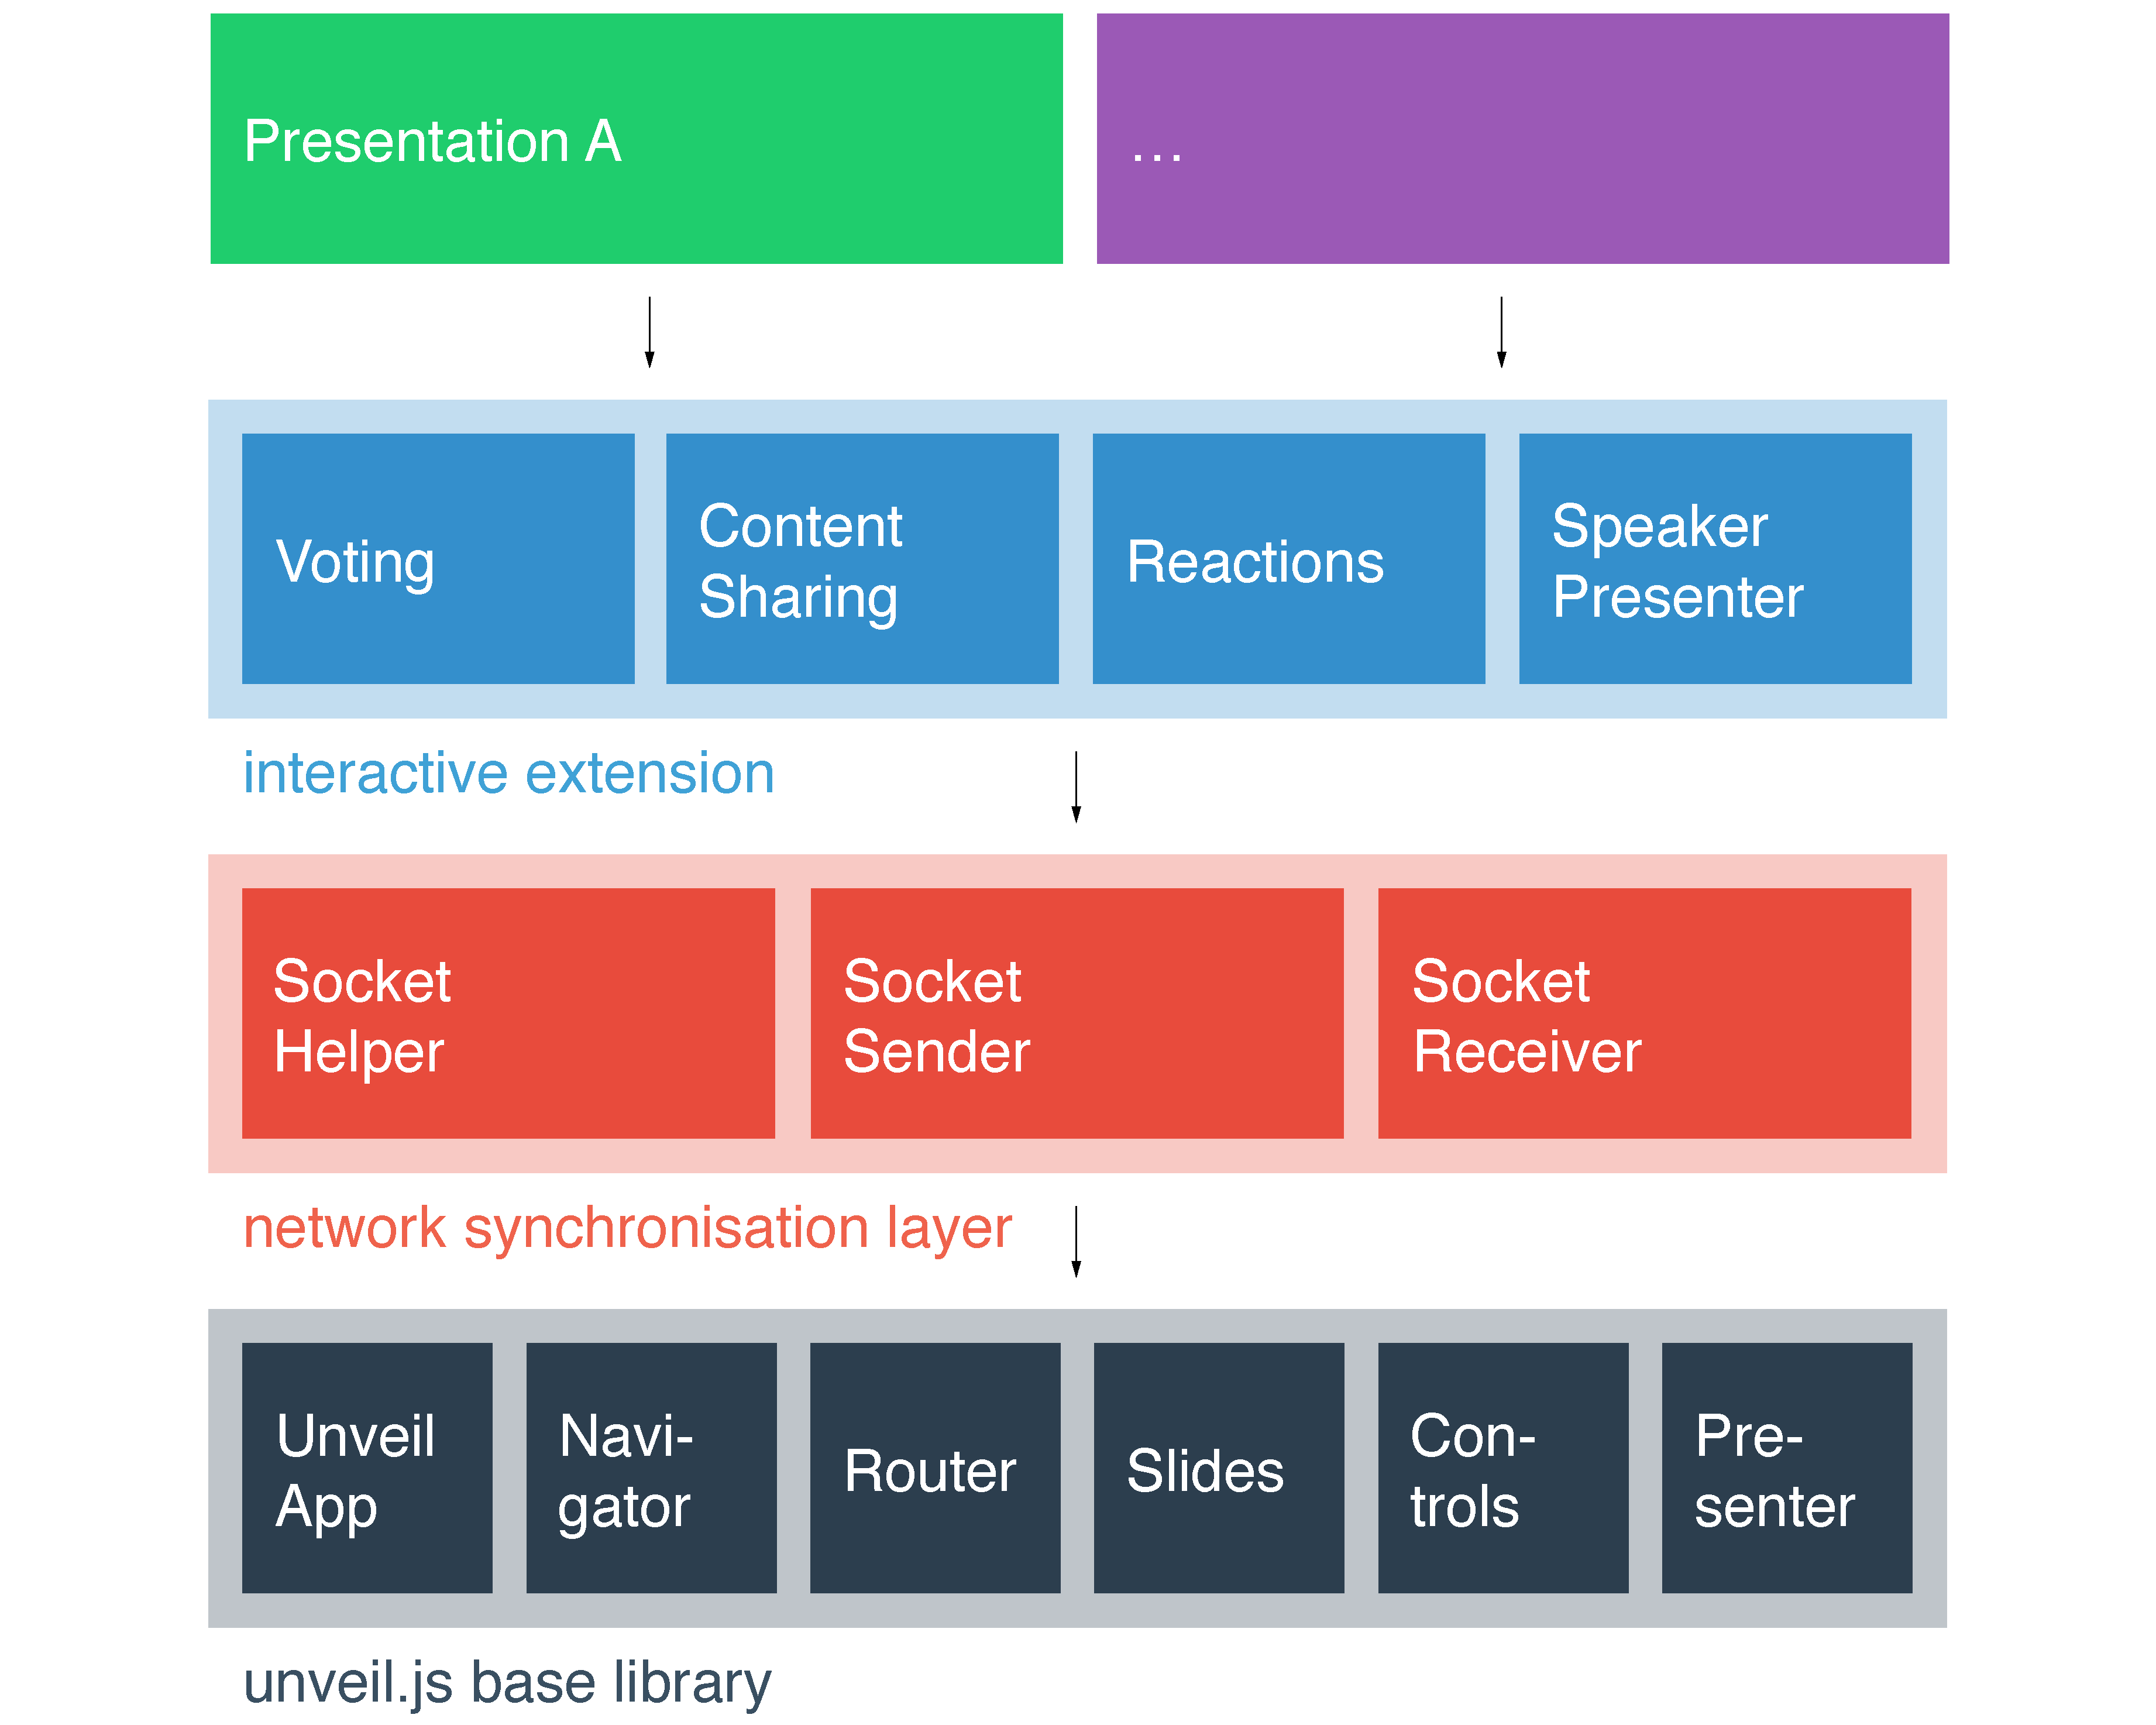
\includegraphics[width=.75\textwidth]{implementation-big-picture}
\caption{Overview of created libraries and their components. Arrows indicate dependencies. At the bottom, the extended version of unveil provides all base functionality. The network synchronisation layer adds support for WebSocket communication with the server, building upon which the interactive extension adds all interactive mechanisms. Any presentation can then use the created libraries.}
\label{fig:implementation-big-picture}
\end{figure}

Like many other projects in this area \cite{Bry:Backstage, Cheng:TreebasedOnlinePresentations, Esponda:ElectronicVotingOnTheFly, Inoue:RealTimeQuestionnaire, Teevan:MobileFeedbackDuringPresentation, Triglianos:InteractiveWebPresentationsImpress}, this project is realised using the web as a platform.
% ADD HERE HOW EVERYTHING IS CONNECTED?!
This has many advantages, from modern web technologies' quick prototyping capabilities to the web's general cross-platform and cross-device nature, the project has benefitted from the dynamicity of the internet and the rapid evolvement of JavaScript over the past years.
Although native sharing features of smartphones cannot be used due to the choice of platform, we believe, the merits that come with this decision outweigh the disadvantages for both users and developers. As no app has to be downloaded, it is easier to bring the audience to use the developed application \cite{Triglianos:InteractiveWebPresentationsImpress}. The major advantage for developers on one hand is the ability to only focus on one platform instead of developing different applications for different operating systems, on the other hand the web is built for rapid prototyping as it is extremely easy and fast to roll out new updates without having to distribute them through the App Store or Play Store and without the need for users to manually update them. Since the JavaScript render layer this software was developed with \cite{react} also offers a library which can cross-compile JavaScript applications to different operating systems \cite{react-native}, the core code could potentially stay almost untouched, should the application be ported to other platforms in the future.

Finally, a few words should also be said about the distribution of this project. Without the vibrant open-source community, many of the frameworks and libraries used in this project would not exist. For this reason, and to give back to the community, all the libraries developed during this project have been published as open-source on GitHub\footnote{\href{https://github.com/irisSchaffer?tab=repositories}{\textsf{https://github.com/irisSchaffer/}}} and are freely available for anyone to use. We concentrated on creating an extensible system for any developer to customiste, adapt, plug into and build interactive presentations with; the only requirement being basic HTML, CSS and JavaScript knowledge.

\section{Project Scope}
\label{sec:implementation-scope}
% What's the general scope of the project? Why is everything on the client and
% not the server? etc.
Before jumping into technical details, the scope of the project should be discussed. As the aim of the present work is to explore ways of incorporating mobile devices into presentation workflows, the goal of the project was to build the mechanisms described in the previous chapters on top of a JavaScript presentation library. As the focus was placed on the interaction possibilities between speaker and audience, the creation of the presentation (e.g. using a graphical user interface) or the management of slides and presentations were out of scope. As with most JavaScript presentation libraries, the resulting application is mainly aimed towards developers, both to extend the libraries further as well as to create presentations, as at least basic knowledge of HTML and CSS is necessary to build slides.

In total, a front end heavy system was created which features several ways of interacting with a presentation, both from mobile and desktop devices. Emphasise was put on mobile-optimised views and navigation possibilities. The end product consists of several, highly customisable libraries which can be combined to a presentation library which synchronises navigation state and state changes between listeners and speaker(s), includes three distinct interfaces for listeners, speakers and projects and offers the possibility to dynamically add content during the presentation. In the following, the general architecture and technologies used in the project will be analysed and described to then discuss implementation details, problems and solutions for the main features.

\begin{figure}
\centering
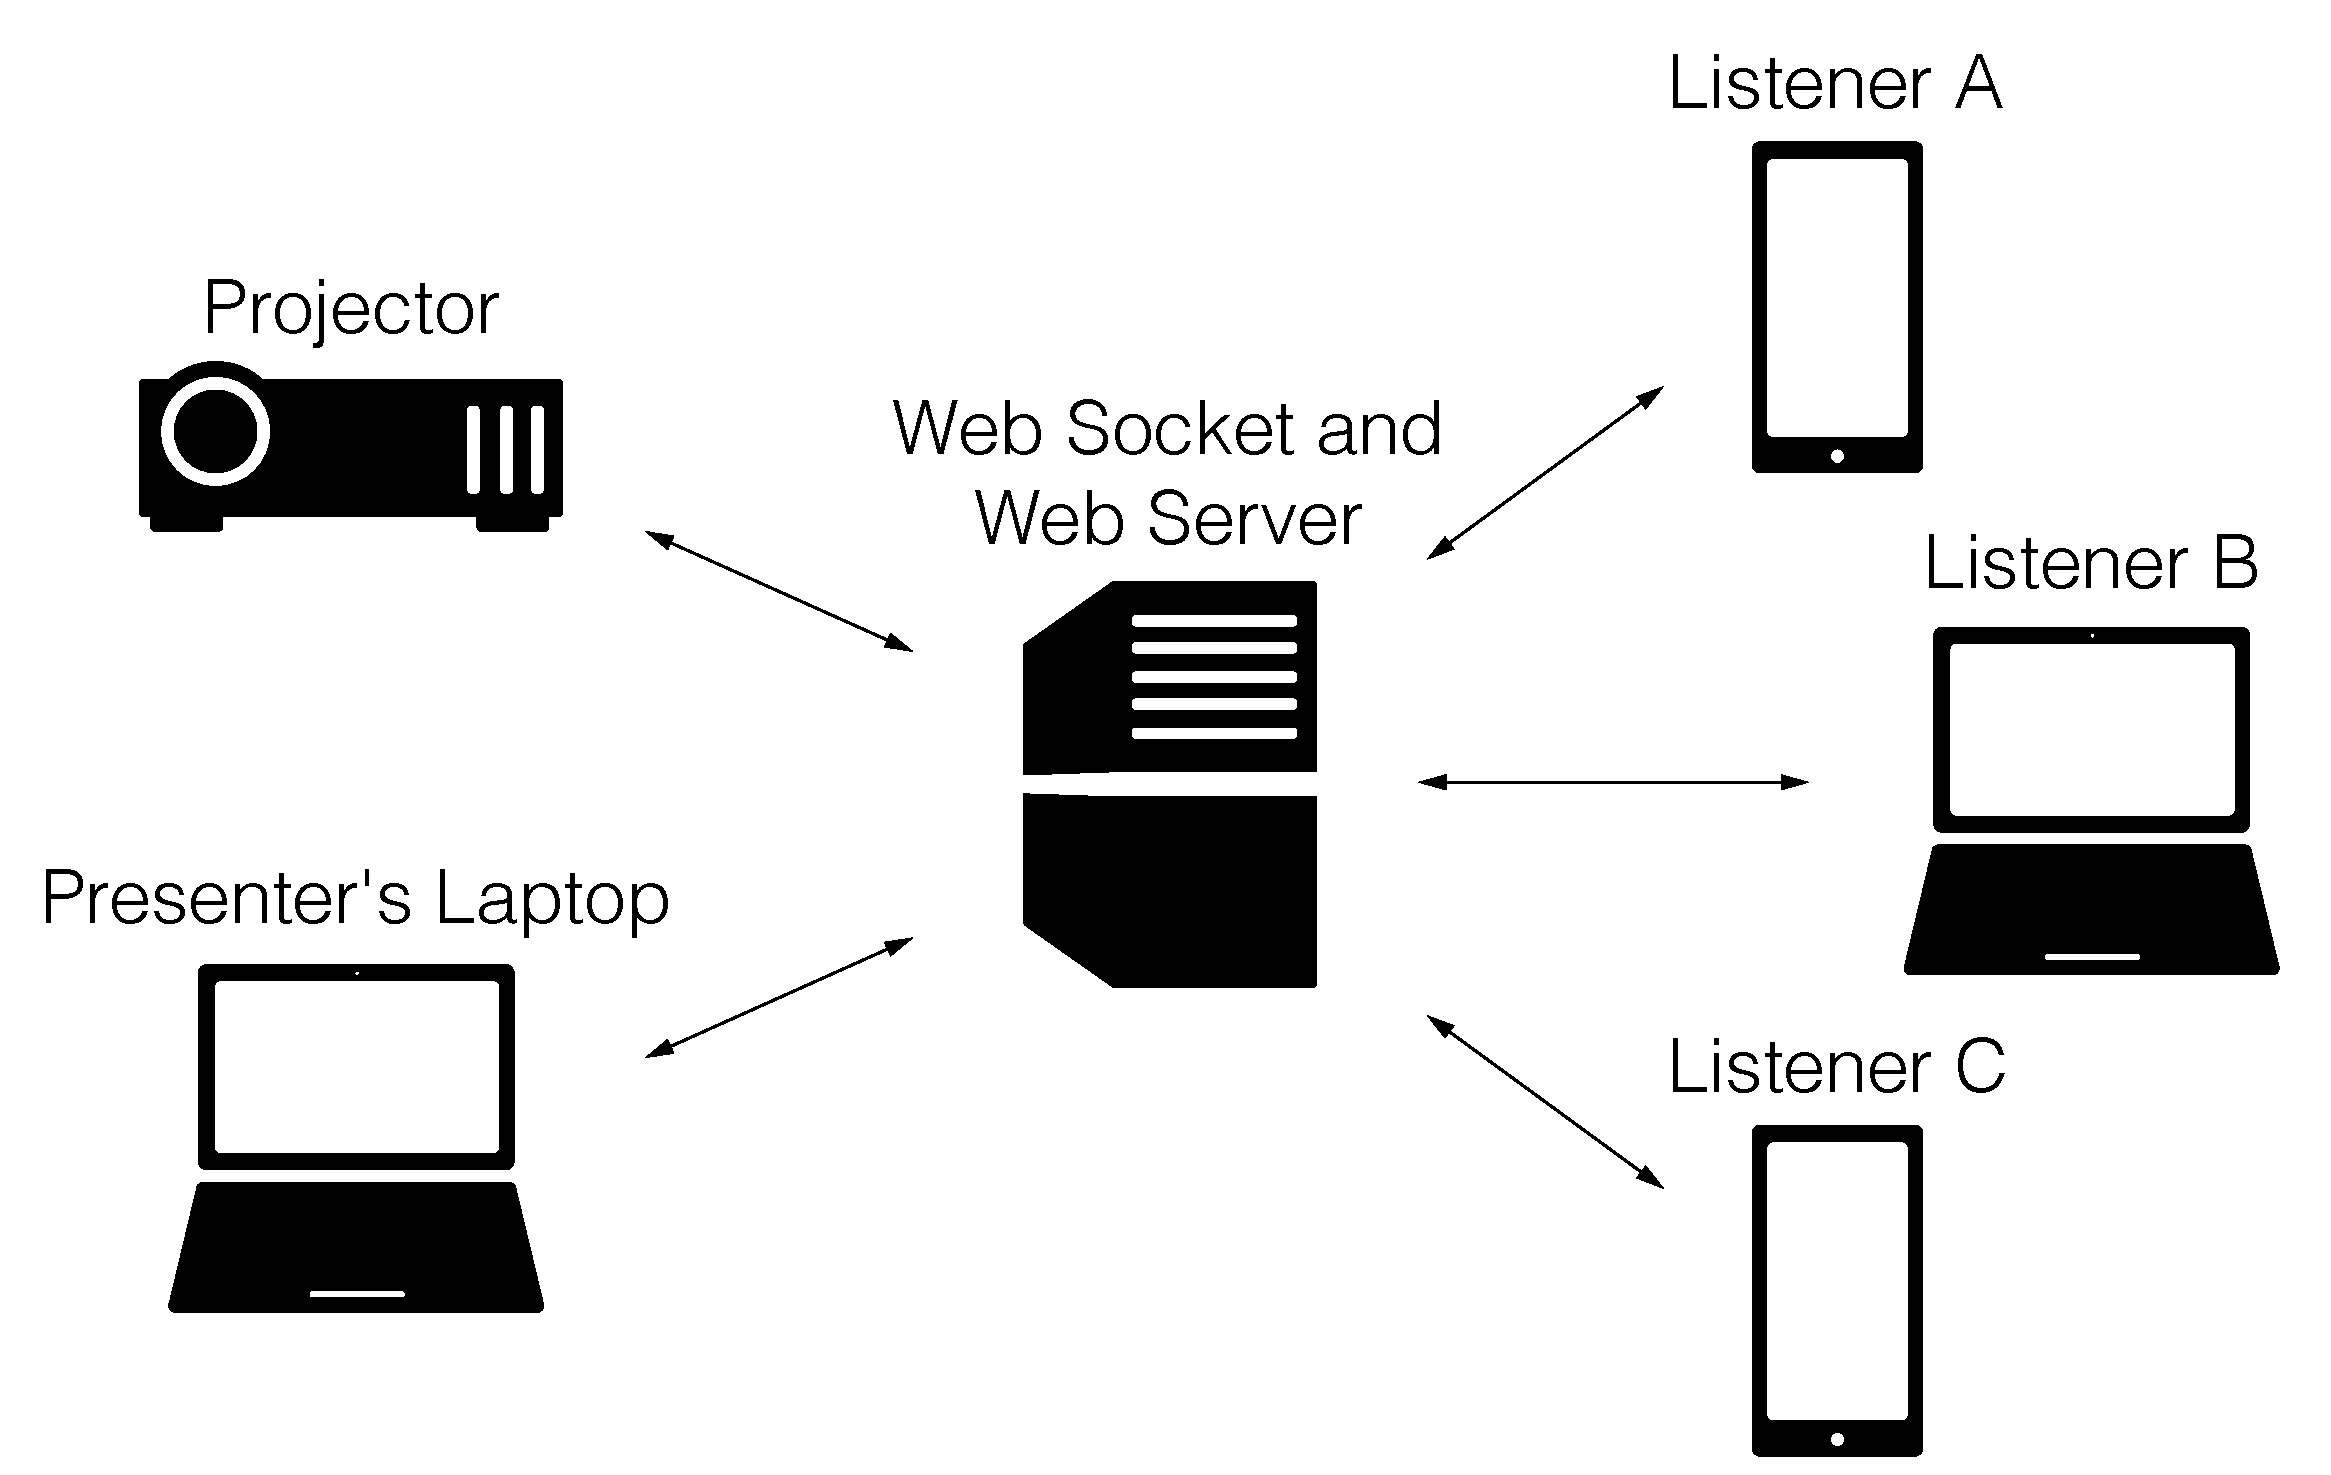
\includegraphics[width=.6\textwidth]{setup}
\caption{Example application setup. A server serves the presentation and connects all clients (presenter devices, listener devices and projector) through WebSockets.}
\label{fig:implementation-architecture-setup}
\end{figure}

\section{Server Architecture}
\label{sec:implementation-server}

In general, the application consists of two parts: the front end web application, run on every client, as well as a web server (see figure \ref{fig:implementation-architecture-setup}). As described in chapter \ref{cha:design}, this server is either publicly-accessible or -- if all listeners have access to the same network -- run on any computer on the local network. While special attention was paid to the front end libraries developed, the server was kept as simple as possible, allowing any developer to work with their own servers and technology stacks. However, the limitation of having such a lightweight and \emph{dumb} server, is that in the current iteration of the prototype all state changes are only persisted on the client-side. although good for testing purposes, as a reset is only a page-reload and clearing of local storage away, this means audience members joining the presentation after any additional slides were added, will not have the same state of the presentation.

The server's two only requirements are on one hand to serve the static web application to all clients, and on the other hand to connect all of these clients to enable the interaction and synchronisation between them using \emph{WebSockets}. This technology was chosen as low response times for all network-requests were paramount and since the technology has already been successfully leveraged in the real-time features of other presentation tools \cite{Inoue:RealTimeQuestionnaire, Triglianos:InteractiveWebPresentationsImpress}. In our server implementation, the presentation is run from a \emph{Node.js} \cite{nodejs} server, using \emph{Express}\cite{express} as a framework. WebSocket support is added using the popular library \emph{socket.io} \cite{socketio}, which a few more words will be said on in section \ref{sec:implementation-network-sync}.
To again emphasise how low the requirements for such a server are, a working example implementation can be found in program \ref{prog:implementation-server-code}. Additionally to this, the server developed for this project also includes a \texttt{lastState}, which holds the last client state which is emitted whenever a new client joins. Once the connection between client and server is established, the server starts broadcasting all incoming requests from any client to all other ones (see figure \ref{fig:implementation-client-server-communication}). These requests are then processed on the clients locally, taking into consideration the mode they are currently in. Wherever possible, the clients optimistically update the interface instead of waiting for the response from the server, to make the application feel even faster.

\begin{program}
\caption{Very simple, possible implementation of a server running this project with Node.js and Express. Wildcard support can be added to socket.io as described in \cite{socket-io-wildcards}.}
\label{prog:implementation-server-code}
\begin{JsCode}
var express = require('express'); var app = express();
var server = require('http').createServer(app);
var io = require('socket.io')(server);

// directory 'client' will be served by server
app.use(express.static(__dirname + '/../client/'));

io.on('connection', function(socket) { // setting up socket io
  socket.on('*', function(event, data) {
    io.emit(event, data);
  });
});

server.listen(9000, function () {
  console.log('Unveil server listening on port 9000!');
});
\end{JsCode}
\end{program}

\section{Front End Technologies}
\label{sec:implementation-technologies}
% Which technologies were chosen and why?
% How do they generally work? To a level on which the reader can
% understand the rest of the implementation details
% A few words about responsive design and media queries would probs be good
% a few words about babel and es6

\begin{figure}
\centering
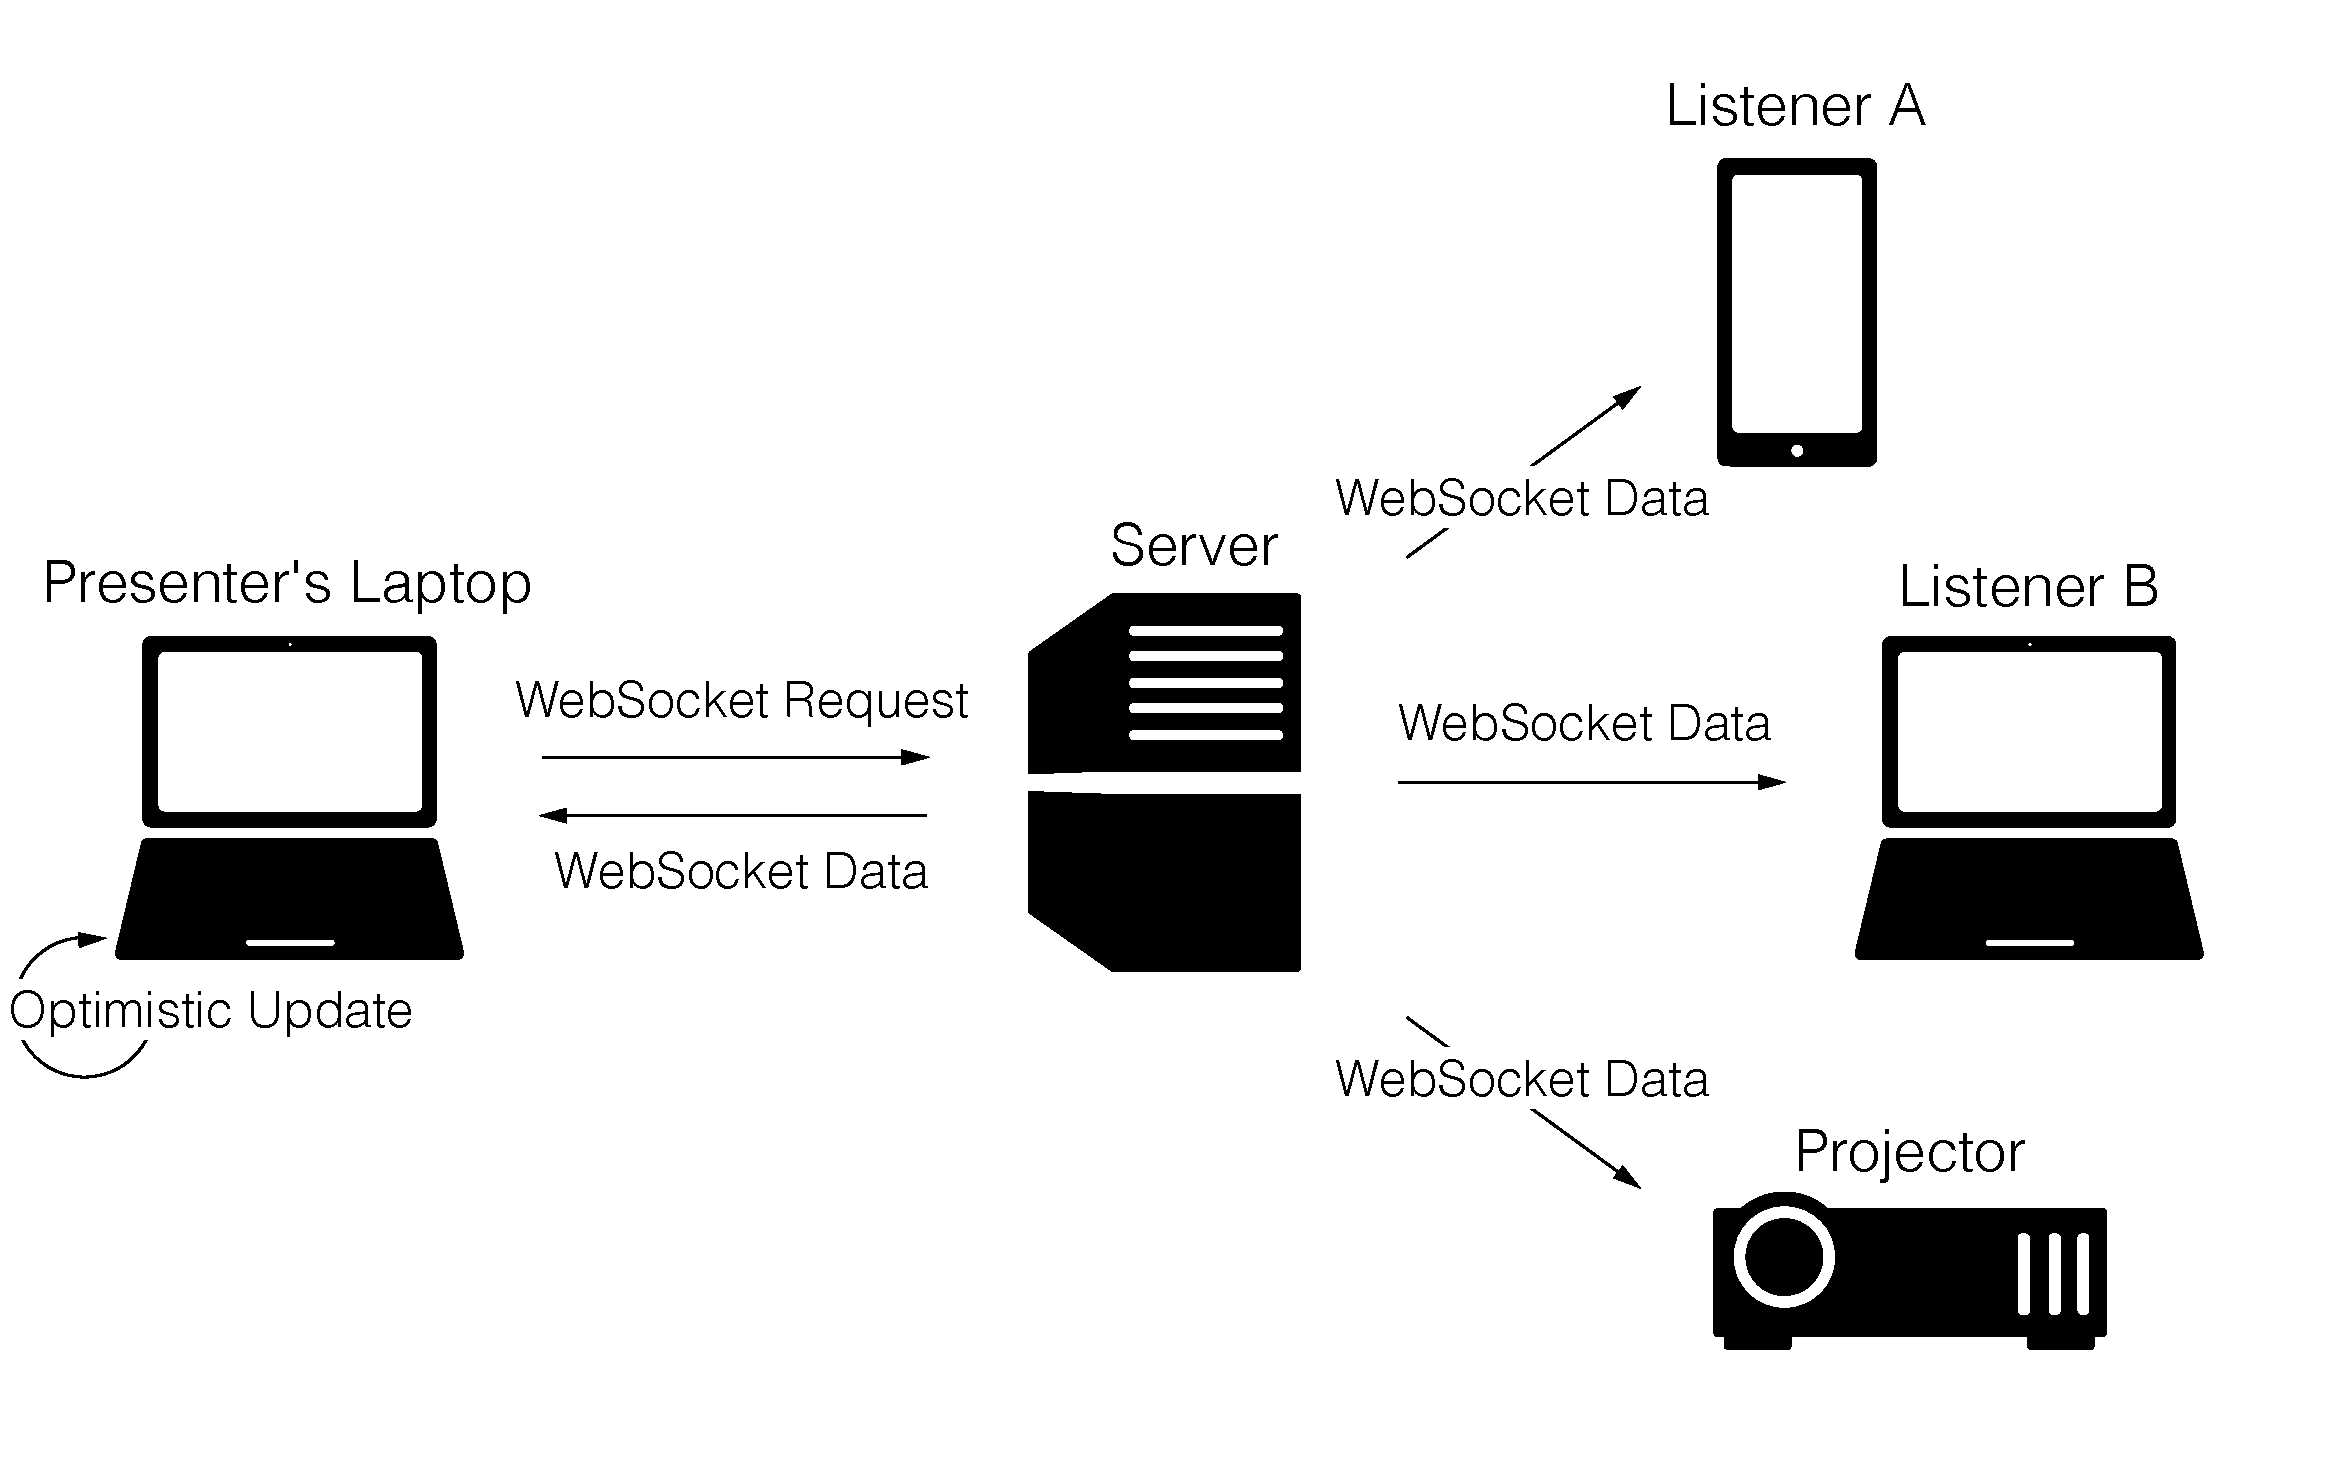
\includegraphics[width=.8\textwidth]{server-communication}
\caption{Client-server communication. The server receives the request from the client and forwards it to all clients.}
\label{fig:implementation-client-server-communication}
\end{figure}

The project generally follows modern best-practices in web development and utilises modern CSS3 and JavaScript features and frameworks. The software is written in ECMA\-Script\-2015, makes use of the \emph{node package manager} (short \emph{npm} \cite{npm}) for managing dependencies and \emph{Babel} \cite{babel} to transpile the code to ECMA\-Script 5. Additonally to relying on CSS3 features, this project also uses \emph{Sass} \cite{sass} as a CSS pre-processor. The listener-interface was developed mobile-first and the speaker-view with mobile in mind; media-queries allow for these optimisations.

The JavaScript library \emph{React} \cite{react} serves as the render framework of choice, additionally applying the \emph{reactive programming} paradigm using \emph{RxJS} \cite{rxjs} to create a simpler interface for event-driven and asynchronous operations. These technologies will now be introduced to the reader shortly, to establish the knowledge-base necessary to understand the then following technical implementation details.

\subsection{ECMAScript2015 and Babel}
\label{sec:implementation-technologies-es6}
% it's a recommendation, but it takes long until browsers implement it and users update their browsers.
JavaScript undoubtly is an integral part of front end web development and since the emergence of server-side JavaScript with Node.js and its package manager npm, has developed into a programming language widely used by web developers \cite{gpm-meta-transcompiler}. Both \emph{PYPL}\footnote{\url{http://pypl.github.io/PYPL.html}} and \emph{TIOBE}\footnote{\url{http://www.tiobe.com/tiobe_index}} programming language indices rank JavaScript among the top 10 programming languages (PYPL at 5, TIOBE at 7 at the time of writing) \cite{gpm-meta-transcompiler}. Stack Overflow's 2015 Developer Survey even places JavaScript as the number 1, most-used programming language with 54.4\% and JavaScript, Node.js and \emph{AngularJS} \cite{angularjs} all three rank amongst the top 5 languages developers expressed an interest in developing with \cite{stackoverflow-developer-survey}.

However, like any front end technology, JavaScript suffers from slow end user adoption, as a multitude of browser versions exist for different devices and operating systems and many people still do not auto-update their browsers. Another factor is the time it takes for browser-vendors to implement new ECMAScript standards (the standard behind JavaScript) and roll out said updates. This is exactly what is happening with the new ECMAScript standard, ECMA-262, commonly known as ECMAScript 2015 or ES6: Although the General Assembly has adopted the new standard in June 2015 \cite{ecma2015}, \emph{Kangax' ECMAScript compatibility tables}\footnote{\url{https://kangax.github.io/compat-table/es6/}} still show a fairly low level of support, especially among mobile browsers. ES6 makes JavaScript easier and more efficient to write by providing new semantics for default values, arrow-functions, template-literals, the spread operator or object destructuring \cite{es6}. It also makes JavaScript safer to develop with and easier to understand with the introduction of block-scoped variables (\texttt{let} and \texttt{const}) and finally offers native support of modules and promises \cite{es6}.
As these features are all included in the new ECMAScript standard, it is safe to assume browser-vendors will implement them in the near future. Until then, developers who want to already make use of them, can \emph{transpile} ECMAScript 2015 code to ECMAScript 5, which is exactly what Babel does. With almost 750,000 downloads in April 2016 \cite{npm-babel} and companies such as Facebook, Netflix, Mozilla, Yahoo or PayPal using this transpiler \cite{babel-users}, Babel is the de facto standard in transpiling to ECMAScript 5 and was also chosen for this project.

\subsection{Reactive Programming}
\label{sec:implementation-technologies-rxjs}

Another problem with JavaScript, although integral part of the reason for its high popularity, is its asynchronous nature. Especially when working with highly interactive parts, the prime example being user interfaces, sequential programming quickly gets too inflexible to handle complex, event-driven applications \cite{reactive-programming-survey}. The same is true for the server where the possibility to concurrently serve a multitude of different clients is paramount. In these cases JavaScript offers \emph{asynchronous callbacks}. These, however, oftentimes execute more asynchronous code and in turn have to wait for another callback to fire, and another one, and another one..., which can result in something known and dreaded by most any JavaScript developer: \emph{Callback Hell} (see programm \ref{prog:implementation-technologies-rxjs-callback-hell}). Since this project has to fulfill many asynchronous tasks and is heavy on the user-interface and thereby JavaScript's event system, it was crucial to find a way of handling this code gracefully. In the following, different ways of handling asynchronous programming are described, the example of an imaginary file upload will be used to demonstrate the differences on code-level:
\begin{enumerate}
\item A file is chosen by the user
\item The file is read by \texttt{FileReader}
\item The file is uploaded
\item The file upload modal is closed with an animation
\item As soon as the animation is over, a success message is rendered
\end{enumerate}

\begin{program}
\caption{\emph{Callback Hell} -- Nested asynchronous callbacks to create a file upload.}
\label{prog:implementation-technologies-rxjs-callback-hell}
\begin{JsCode}
onFileChange(event) {
  fileReader.readAsDataURL(event.file, (content, error) => {
    uploadFile(content, (response, error) => {
      this.refs.modal.close(() => {
        updateSuccessMessage(response)
      })
    })
  })
}
\end{JsCode}
\end{program}

\noindent Different approaches have been employed to lower the hurdle of writing asynchronous code, one of them being \emph{promises}: A promise is a value, yet to be computed \cite{reactive-vs-promises}. A promise can be a) pending (if it has not been assigned a value yet), b) resolved (if it has been assigned a value) or c) rejected (if an error occurred). With ECMAScript 2015 promises, these objects can then be queued using the \texttt{then} keyword, to execute asynchronous code in a certain sequence (see programm \ref{prog:implementation-technologies-rxjs-promises}).

\begin{program}
\caption{\emph{Promises} -- File upload example using ECMAScript 2015 promises.}
\label{prog:implementation-technologies-rxjs-promises}
\begin{JsCode}
onFileChange(event) {
  fileReader
    .readAsDataURL(event.file)
    .then(uploadFile)
    .then((response) => {
      this.refs.modal.close(() => promise.resolve(response))
    })
    .then(updateSuccessMessage(response))
}
\end{JsCode}
\end{program}

\noindent However, promises can still create nested callbacks, especially when chaining promises that rely on other promises' resolution \cite{reactive-vs-promises}. This is where \emph{reactive programming} shines: The reactive programming paradigm works with streams of events, in which every event is handled as a new value and all other parts depending on that value are re-computed upon arrival of such new value. Bainomugisha et al.  \cite{reactive-programming-survey} use the illustrative example of a simple addition to demonstrate this: In sequential programming, $c$ the expression $c = a + b$ with $a = 1$ and $b = 2$ will always be $3$, until assigned a different value. With reactive programming, however, should $a$ or $b$ change, the value of $c$ is automatically re-computed.
JavaScript does not directly support reactive programming, but more functional languages like \emph{Elm} \cite{elm} which can be transpiled to JavaScript, do. Another way of adding reactive programming concepts to JavaScript is using a library, such as \emph{Bacon.js} \cite{baconjs} or the one chosen for this project, \emph{ReactiveX}\footnote{\url{http://reactivex.io/}}. ReactiveX provides libraries for a multitude of different programming languages, C\#, C++, Java and of course JavaScript among them. The latter, called \emph{The Reactive Extensions for JavaScript} or short \emph{RxJs} \cite{rxjs}, allows for the processing of event streams (\emph{Observables}) as if they were simple JavaScript arrays. Instead of writing sequential code, method after method, if asynchronous or not, is applied to every element in the incoming event stream, using the array-methods such as, most notably and well-known, \texttt{map} (to apply a method to every element in the incoming stream) and \texttt{filter} (to only let a subset of events pass) (see programm \ref{prog:implementation-technologies-rxjs}).

\begin{program}
\caption{\emph{RxJS} -- File upload example with reactive programming in RxJS.}
\label{prog:implementation-technologies-rxjs}
\begin{JsCode}
Observable.fromEvent('change', fileInput)
  .pluck('file') // pluck event.file
  .map(fileReader.readAsDataURL)
  .map(uploadFile)
  .do(() => this.refs.modal.close)
  .subscribe(updateSuccessMessage)
\end{JsCode}
\end{program}

Additionally to Observables, RxJs also knows \emph{Subjects}, which combine both a source of events and a consumer of such. Subjects are Observables but at the same time also Observers and can be used to broadcast values to several consumers \cite{rxjs}.

\subsection{React}
\label{sec:implementation-technologies-react}
% explain base concept of having re-usable components and how they are defined!
% get some HTML code in there :)

As this project focuses on the front end, a mature JavaScript library for front end rendering was needed. After previous experience with the big and complex but slow AngularJS, and because of promising performance benchmarks \cite{react-benchmarks} and simply to explore new JavaScript libraries, React was chosen for the rendering layer of this application. Since Facebook started developing React in 2013, it has challenged existing approaches and set new standards in front end web development \cite{introduction-to-react}. Instead of creating an entire MVC framework for the front end, React really concentrates on the view by offering a way of creating independent, lightweight view components. This gives React the huge advantage of beating other front end frameworks in performance benchmarks by far \cite{react-benchmarks}. Moreover, \emph{React Native} \cite{react-native}, which uses the same component-based system, makes it possible to port applications to different mobile operation systems.

To define how each of these re-usable, lightweight components is displayed, they implement a \texttt{render} method, returning JSX \cite{jsx}. The communication with other components happens through \emph{properties} (\texttt{props}), which are passed into the component as XML attributes. Their own internal state, which can be manipulated e.g. through user interactions, is maintained in the \texttt{state} member \cite{react-docu}. Every state (internal) or property (external) change causes a re-render of the component, an example \texttt{HelloWorld} component can be found in program \ref{prog:implementation-technologies-react-state}.
%
\begin{program}
\caption{Example code snippet using properties and state in a React component. Whenever the text input changes (i.e. a user types something), the state will be updated and the component re-rendered. The component can be used in other components as \texttt{<HelloWorld greeting=''Hi''/>}.}
\label{prog:implementation-technologies-react-state}
\begin{JsCode}
export default class HelloWorld extends Component {
  static propTypes = { greeting : PropTypes.string }
  static defaultProps = { greeting : 'Hello' }

  constructor(props) {
    super(props)
    this.state = { name : 'World' }
  }

  const render = () => (
    <div>
      <h1>{this.props.greeting} {this.state.name}!</h1>
      <input value={this.state.name} onChange={(name) => this.setState({ name })} />
    </div>
  )
}
\end{JsCode}
\end{program}
%
These updates, as well as construction and destruction of components are handled in \emph{lifecycle methods} \cite{react-docu}.

As an end note on React, and a transition to the core presentation library, it should be added that React components can be nested arbitrarily deep, effectively creating semantic XML syntax which is directly linked to the rendering of the components. To make it as easy as possible for other developers to use the created libraries and components, presentations are built just as a usual HTML page, using these semantic XML tags, as will be shown in chapter \ref{cha:results}.

\subsection{unveil.js}
\label{sec:implementation-technologies-unveil}
% explain how this was developed together with Leandro, explain general parts like router, navigator, UnveilApp
% Give overview over controls in here.
% Also talk about the mobile style sheets / responsive design and the TouchControls, which I also implemented alone.
% (mention that this part is unit tested with jest(https://facebook.github.io/jest/))
Although not initially planned, due to several shortcomings of other presentation libraries, this project builds upon the open-source JavaScript library \emph{unveil.js} \cite{unveil}, which we developed prior to this project and extended and adapted in an own fork \cite{unveil-fork} during the project. While other alternatives, such as \emph{impress.js} \cite{impressjs} or the popular \emph{reveal.js} \cite{revealjs}, exist, extensive research showed that neither of the two libraries offers the flexibility necessary to easily implement the discussed interactive mechanisms. They both were not built unleashing modern web technologies' full potential and practically consist of one big file of JavaScript, handling all functionality. We therefore decided to build our own presentation platform.

Generally, unveil.js, like impress.js and reveal.js, is a library with which online presentations can be built. All three do not require a web server and can therefore be statically, and also locally served. Instead of building the presentation using a graphical user interface, all slides, transitions and styling are defined in HTML and CSS, meaning the presenter has to be familiar with basic front end web development techniques. Thanks to the use of React, unveil.js, in contrast to reveal.js and impress.js, however, does not depend on the usage of class names to identify the slide structure, but instead can make full use of semantically-named components, such as \texttt{<Slide/>} or \texttt{<Notes/>}. More details about the usage of unveil will be covered in chapter \ref{cha:results}.

Like reveal.js, unveil.js operates on a $2$-dimensional slide-space: Every slide can have a next and previous slide in $x$ (main slide), as well as in $y$-direction (sub-slide). To generate the $y$ axis, slides are nested in other slides.
To be able to identify slides from a URL, slides have an optional unique name as well as an index in the slide-tree. Both the index and the name can be used to link to a certain slide, making it possible to share not only a whole presentation but also a certain slide.

The core of unveil.js is \texttt{UnveilApp}, which all slides and sub-slides are nested in. This component configures and sets up the entire application based on optional configuration passed in as properties. There are a few concepts we introduced jn unveil.js to allow for maximal extensibility and adaptability, namely \emph{presenters}, \emph{controls} and \emph{modes}:
%
\begin{itemize}
\item \textit{Presenters} define the way the current slide is rendered, e.g. where to display controls, if to show notes, or whether to rencer upcoming slides.
\item \textit{Controls} control a part of the application. One example would be the navigating from one slide to the next using the arrow keys on the keyboard.
\item \textit{Modes} are what allow a speaker to have a different presenter and controls from an audience member. Each mode defines its own presenter and set of controls, the mode is determined by the url query parameter \texttt{mode}.
\end{itemize}
This allows anybody using unveil.js to define or overwrite modes, presenters and controls and thereby extend the base library as they wish. A few of these are already defined in the base library, namely a default \texttt{Presenter}, \texttt{UIControls} to navigate using buttons, \texttt{KeyControls} to navigate using the keyboard and \texttt{TouchControls} to navigate with swipe-gestures on touch screens. In chapter \ref{cha:results}, modes for the audience (\texttt{de\-fault}), the speak\-er (\texttt{speak\-er}) and for use on the projection device (\texttt{projector}) will be set up.

\begin{figure}
\centering
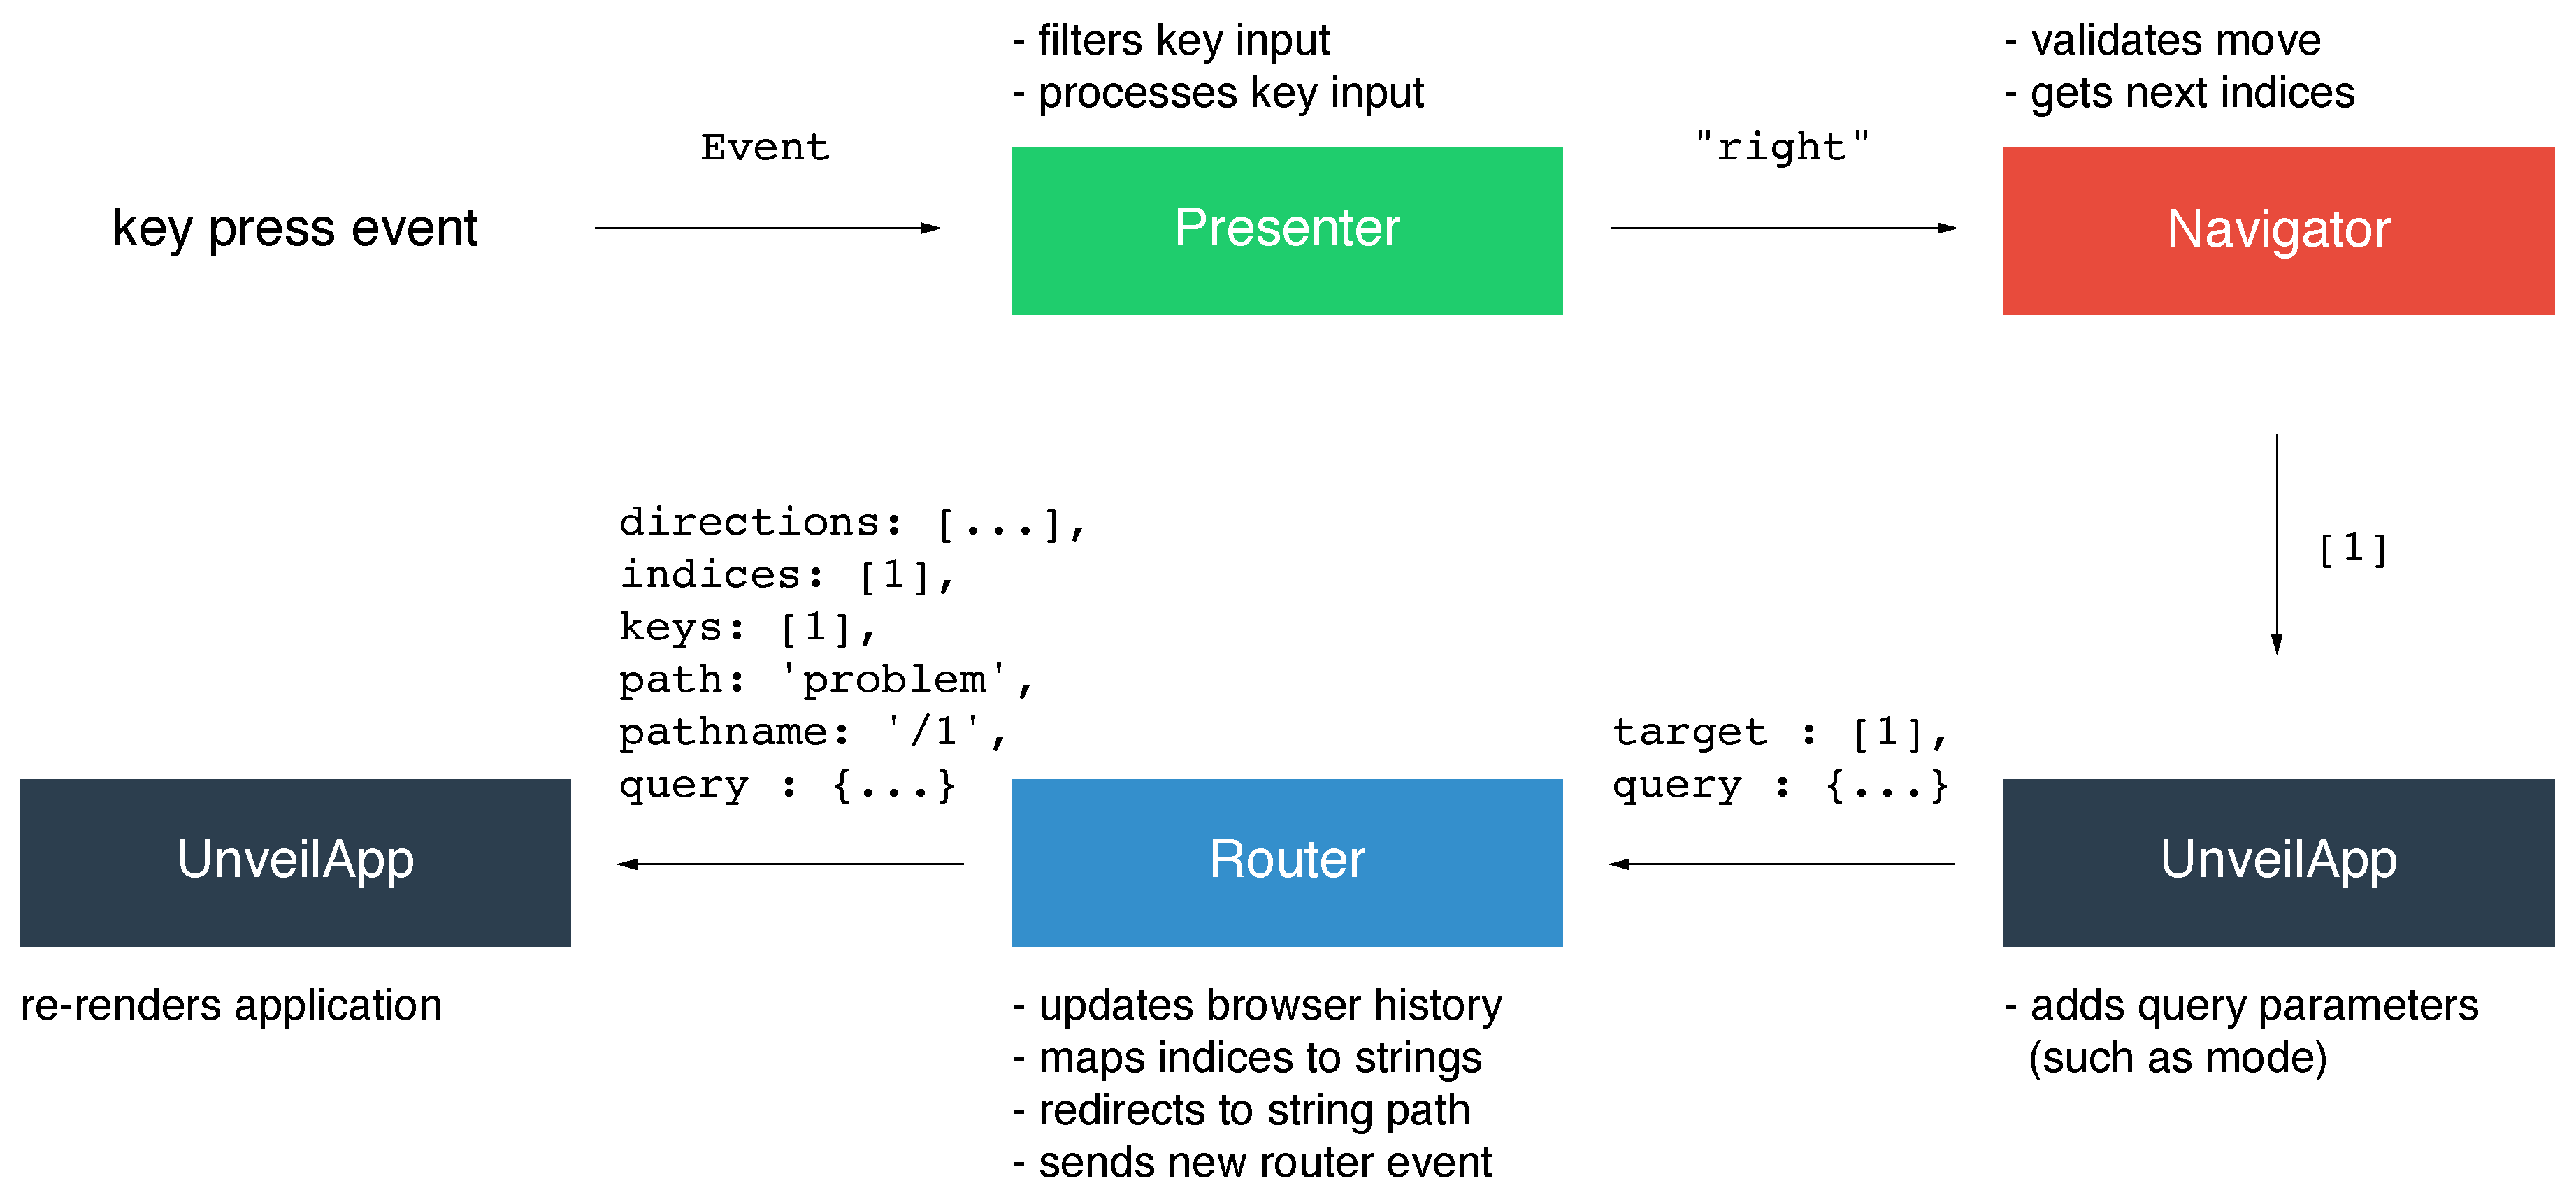
\includegraphics[width=1\textwidth]{navigation-pipeline}
\caption{Navigation pipeline from user's key press to re-render of the presentation. The monospaced text next to the arrows symbolises the data transmitted. \texttt{KeyControls} listen for key events and process them, to then send a navigation request to go \emph{right} to the \texttt{Navigator}. This component then maps the direction to the next slide's indices ($1$). \texttt{UnveilApp} then adds other information necessary for the \texttt{Router}, which then is responsible for updating the browser history, mapping the indices back to a human readable url and sending out a new router event. In the end \texttt{UnveilApp} receives this event and re-renders the presentation.}
\label{fig:implementation-technologies-unveil-navigation}
\end{figure}

For these controls and the entire presentation to be navigatable, \texttt{Un\-veil\-App} is responsible for the creation of two very important classes: \texttt{Router} and \texttt{Navigator}. These can be defined outside and passed into \texttt{UnveilApp} as properties, allowing other developers to customise their navigation logic.
%
The \texttt{Router} is the class handling everything connected to the current url. It receives the slide-tree and can compute the indices of a slide by its name and vice versa. Whenever the browser history changes, the router finds the corresponding slide-indices, computes an array of possible directions to go into from this slide and propagates the event to \texttt{UnveilApp}, which can then re-render the application.
\texttt{Navigator}, in turn, receives these directions and is responsible for the mapping of directions (\emph{left}, \emph{right}, \emph{up}, \emph{down}) to slide-indices. Controls know the navigator and can push new directions to the navigator subject, thus starting the navigation process described in detail in figure \ref{fig:implementation-technologies-unveil-navigation}.

\section{Project Structure}
\label{sec:implementation-structure}
% A graphic explaining how the repos are built on top of each other would be great
% Which repos do I have and what do they include functionality-wise?
% explain why different repos and how they are all own npm packages that can easily be included in other projects

As the puropose of this project was not only to experiment with different ways of interacting with presentations using mobile devices, but also to create something worthwhile and contribute back to the vibrant open-source community, the project is enitrely open-source and separated into different repositories. These can be installed using npm, therefore allowing developers to rely only on the parts they really need. An overview can be found in the beginning of this chapter in figure \ref{fig:implementation-big-picture}.

\paragraph{Extended unveil.js:} As discussed in section \ref{sec:implementation-technologies-unveil}, the project is based on the library unveil.js \cite{unveil}. During the development of the project, certain parts of the base library were improved to allow for even easier extensibility and new presentation logic was added. This happened in a fork of the original library, which will be examined in section \ref{sec:implementation-unveil}.

\paragraph{Network Synchronisation Layer:} The first library of direct importance for the interaction between speaker and audience through personal devices is \textit{unveil-network-sync} \cite{unveil-network-sync}. This rather small library relies on unveil.js and is responsible for connecting the client and the server through web sockets and enables the synchronisation of the current slide displayed between speaker, audience and projector. The implementation of the features will be discussed in detail in section \ref{sec:implementation-network-sync}.

\paragraph{Interactive Extension:} As the name already suggests, this library is at the core of the present thesis: It includes a dedicated presenter for the speaker, implements the insertion of additional slides and subslides and by that allows the audience to share content with the presentation. Reactions, the voting mechanism, as well as the creation of new votings on-the-fly, also live within this library. The repository, called \emph{unveil-interactive} \cite{unveil-interactive} relies on unveil-network-sync for the socket-interaction and will be covered in section \ref{sec:implementation-interactive} of this chapter.

\paragraph{Server and Example Presentation:} The last repository connected to this thesis \cite{unveil-client-server} includes a simple server as well as a real-world example of a presentation. In this chapter, one section was already dedicated to the server (\ref{sec:implementation-server}), a short introduction into the usage of the developed library will be given in chapter \ref{cha:results}.

\section{Extended unveil.js}
\label{sec:implementation-unveil}
% Add screenshots from biiiiiiig screen :)
The biggest adaptions and additions were necessary in the main component \texttt{UnveilApp}. A state subject was added to allow all components in the presentation to interact with the application. This subject receives an event with type and data and depending on this type starts a certain state change. Two of these state events are the \texttt{state/navigation:enable} and \texttt{state/navigation:disable} events, which set a state-variable \texttt{navigatable} to true or false. This variable is used in the controls to determine navigatability, therefore making it possible to keep the audience locked to a slide, e.g. during votings.
To make it possible for the audience to add subslides, as well as to dynamically add votings on-the-fly, another event is \texttt{state/slide:add}. It includes what slide to add (content), how (subslide or main slide) and where (under or after which slide). On occurence of this event, the slide-tree has to be re-built, the router and navigator re-started and the whole presentation re-rendered, which the library also had to be prepared for. A complete list of all state events and who they are emitted by and listened to can be found in figure \ref{fig:implementation-events-network-sync} and \ref{fig:implementation-events-interactive}.

\begin{figure}
\centering
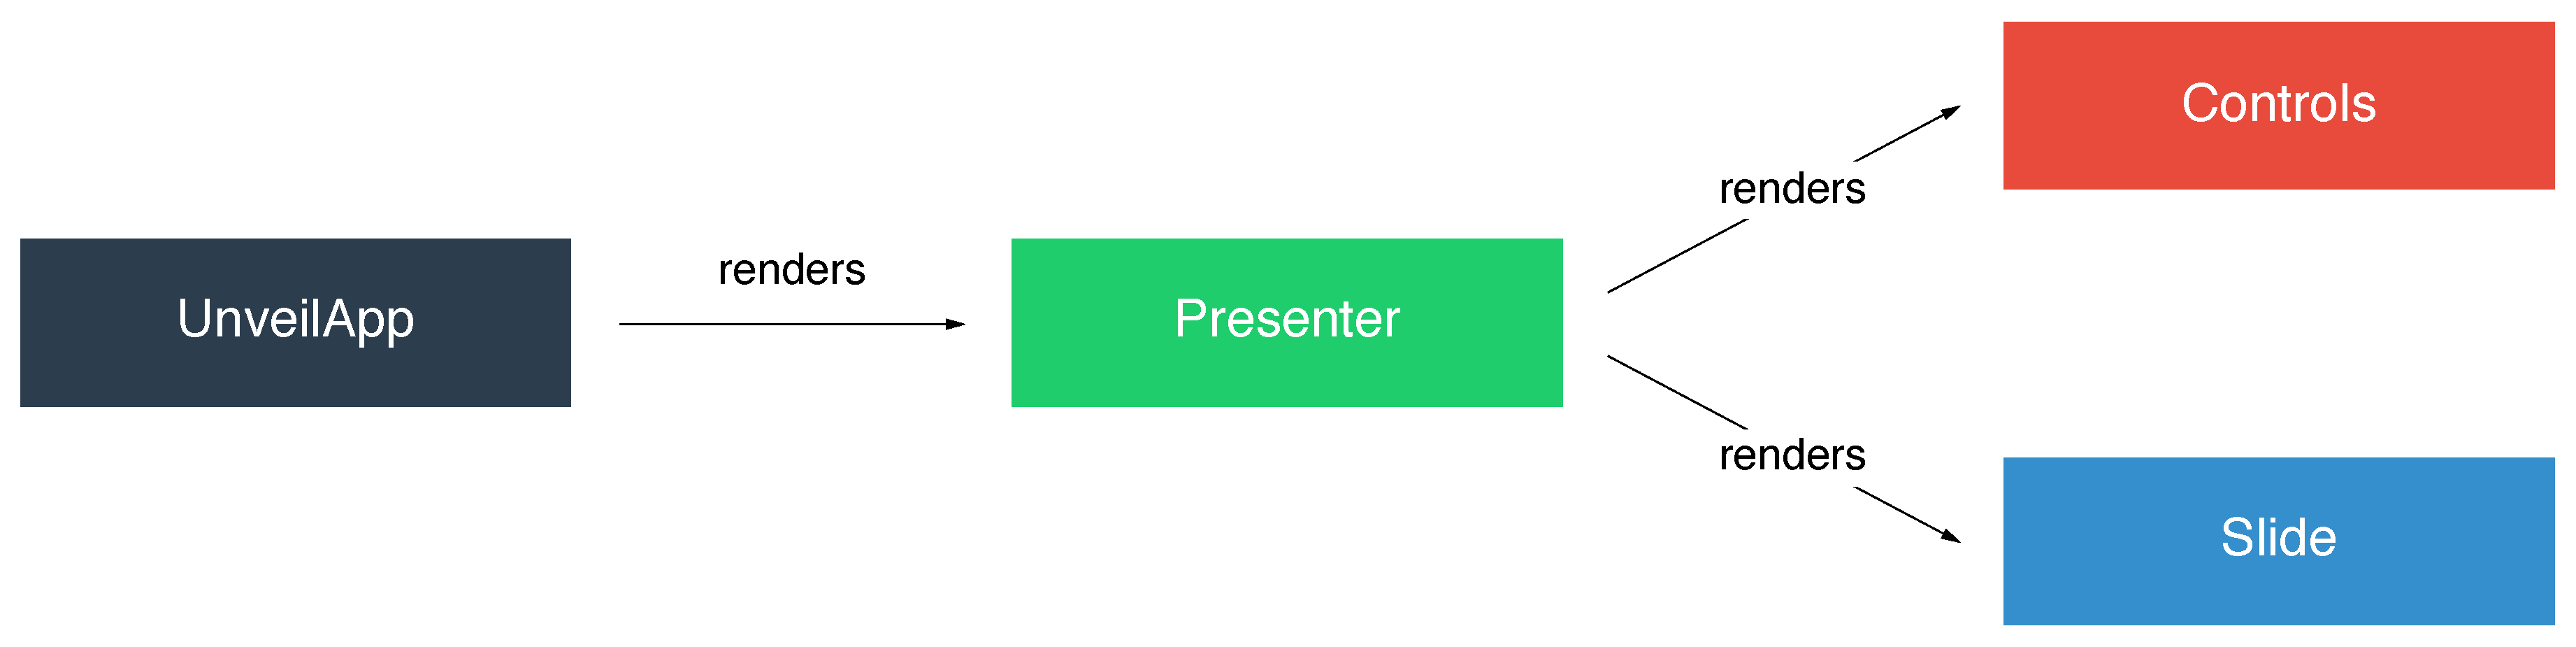
\includegraphics[width=1\textwidth]{render-pipeline}
\caption{Overview over the render-flow of the application in the extended version of unveil.js. \texttt{UnveilApp} renders the presenter, which then takes care of rendering the (current) slide and all controls.}
\label{fig:implementation-unveil-render-pipeline}
\end{figure}

Another adaption in \texttt{UnveilApp} is the introduction of the \texttt{context} object: Additionally to state and properties, there is a third way of communicating between components in React, called \emph{context}. Instead of having to pass properties from one nested component to the other, every child component can access the context of its parents. The navigator, needed in the controls, was formerly passed from \texttt{UnveilApp} to the controls through several layers. Using context, \texttt{UnveilApp} now defines a number of different variables which are available through context, including current slide and router state, navigator, mode and the state subject discussed in the last paragraph. This makes it easy for new controls and presenters to access the data they need without other layers knowing about them or having to define them.
This adaption was partly due to a change in the render hierarchy: Formerly, \texttt{UnveilApp} itself rendered the presenter (which rendered the current slide) and the controls. However, the presenter needs to be able to also control the rendering of controls (see figure \ref{fig:implementation-unveil-render-pipeline}), adding another layer between the rendering of controls and \texttt{UnveilApp}.

Another part that was added to the unveil.js base library is the \texttt{Notes} component. It allows adding speaker notes to each slide (see program \ref{prog:usage-presentation-creation}). These, however, are not rendered by the slide, but by the presenter, as will be shown in section \ref{sec:implementation-interactive}. One more important new feature is the possibility to configure the next slide in a certain direction (left/right/up/down) and therefore allow for jumping into different branches of the presentation, thus making a presentation even more interactive. The following code, for example
%
\begin{JsCode}
  <Slide name="start" left={[0]}>
    ...
  </Slide>
\end{JsCode}
%
means a navigation \emph{left} (left arrow key pressed, swipe left etc.) will not go to the previous slide defined in the slide-tree, but rather jump to the first slide (of index $0$).

\section{Network Synchronisation Layer}
\label{sec:implementation-network-sync}

\begin{figure}
\centering
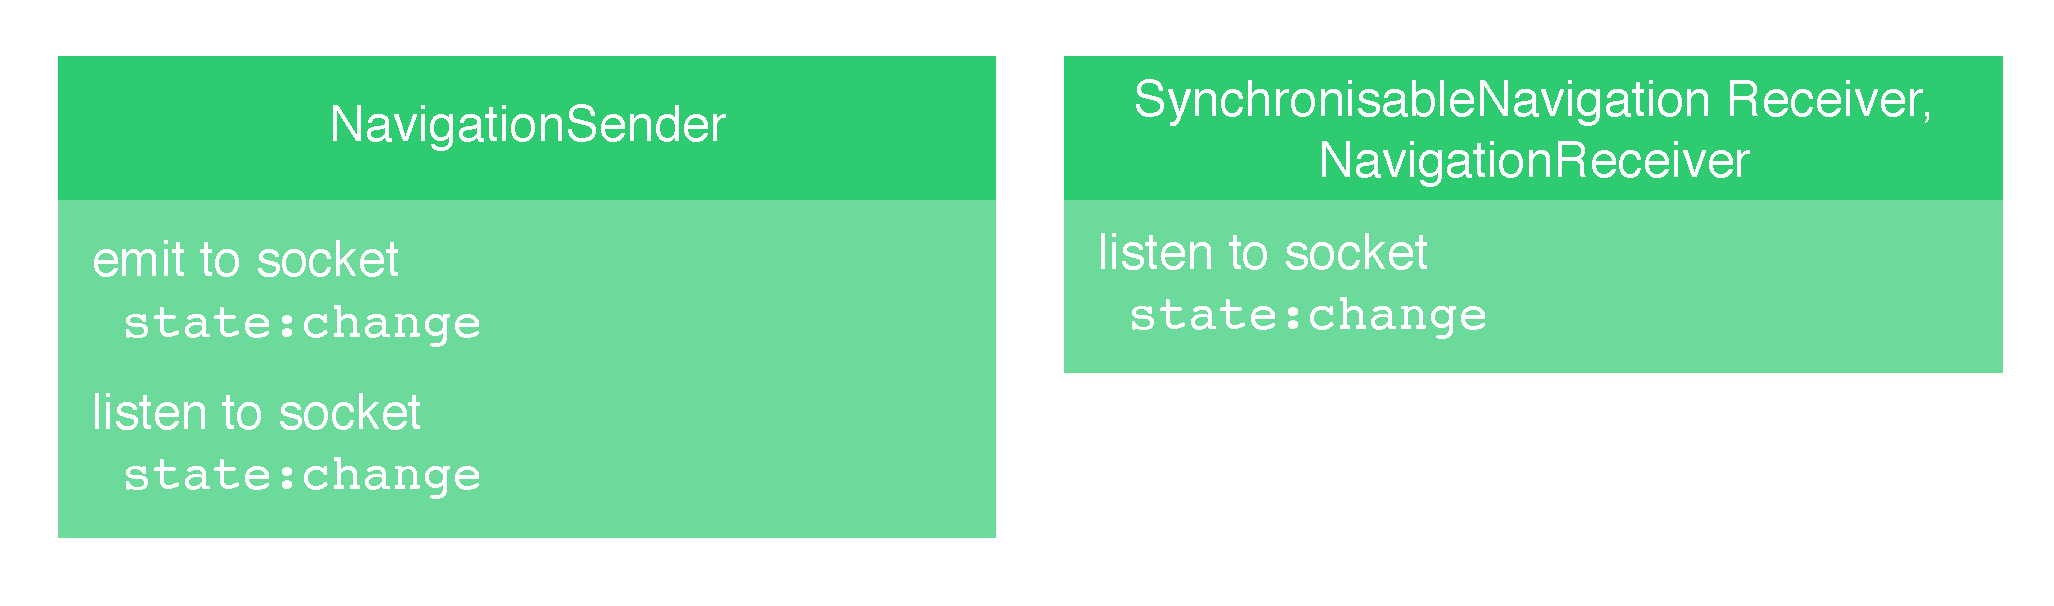
\includegraphics[width=.66\textwidth]{events-network-sync}
\caption{State and socket events sent and consumed by controls in the network synchronisation layer.}
\label{fig:implementation-events-network-sync}
\end{figure}


% Mention problems with socket io here! --> Corporate firewalls can block socket io entirely, etc.
As mentioned before, the network synchronisation layer is responsible for the communcation between server and client using WebSockets. These are created using socket.io, a library which also provides fallbacks for browsers that do not support WebSockets yet. However, the library also has a few drawbacks, especially when it comes to corporate networks. As Rob Britton describes in \cite{socketio-problems}, socket.io seems to have problems getting through firewalls and can be blocked by some anti virus applications.
As mobile browser support was essential for this project, after some consideration, we still decided in favour of this library.

The socket is created by the speaker in the main entry point of the presentation by passing the IP-address of the WebSocket server to the function \texttt{createSocket}, which is directly exposed by \texttt{unveil-network-sync}. Internally the socket connection to the server is established and the then exposed as a singleton, so every component uses the same connection. Inside all controls communicating with the socket server, this connection can be imported through \texttt{SocketIO}, which internally retrieves the singleton:

The connection can then be used to listen to events or to emit them. Like the state subject events, the socket.io events used in this library follow the naming convention of scoping the object targeted in by the event separated by slashes, followed by a colon and the name of the action, e.g. \texttt{state:change} or \texttt{state/slide/voting:start}. The list of all current socket events, together with state events can be found in figure \ref{fig:implementation-events-network-sync}.

\begin{figure}
\centering
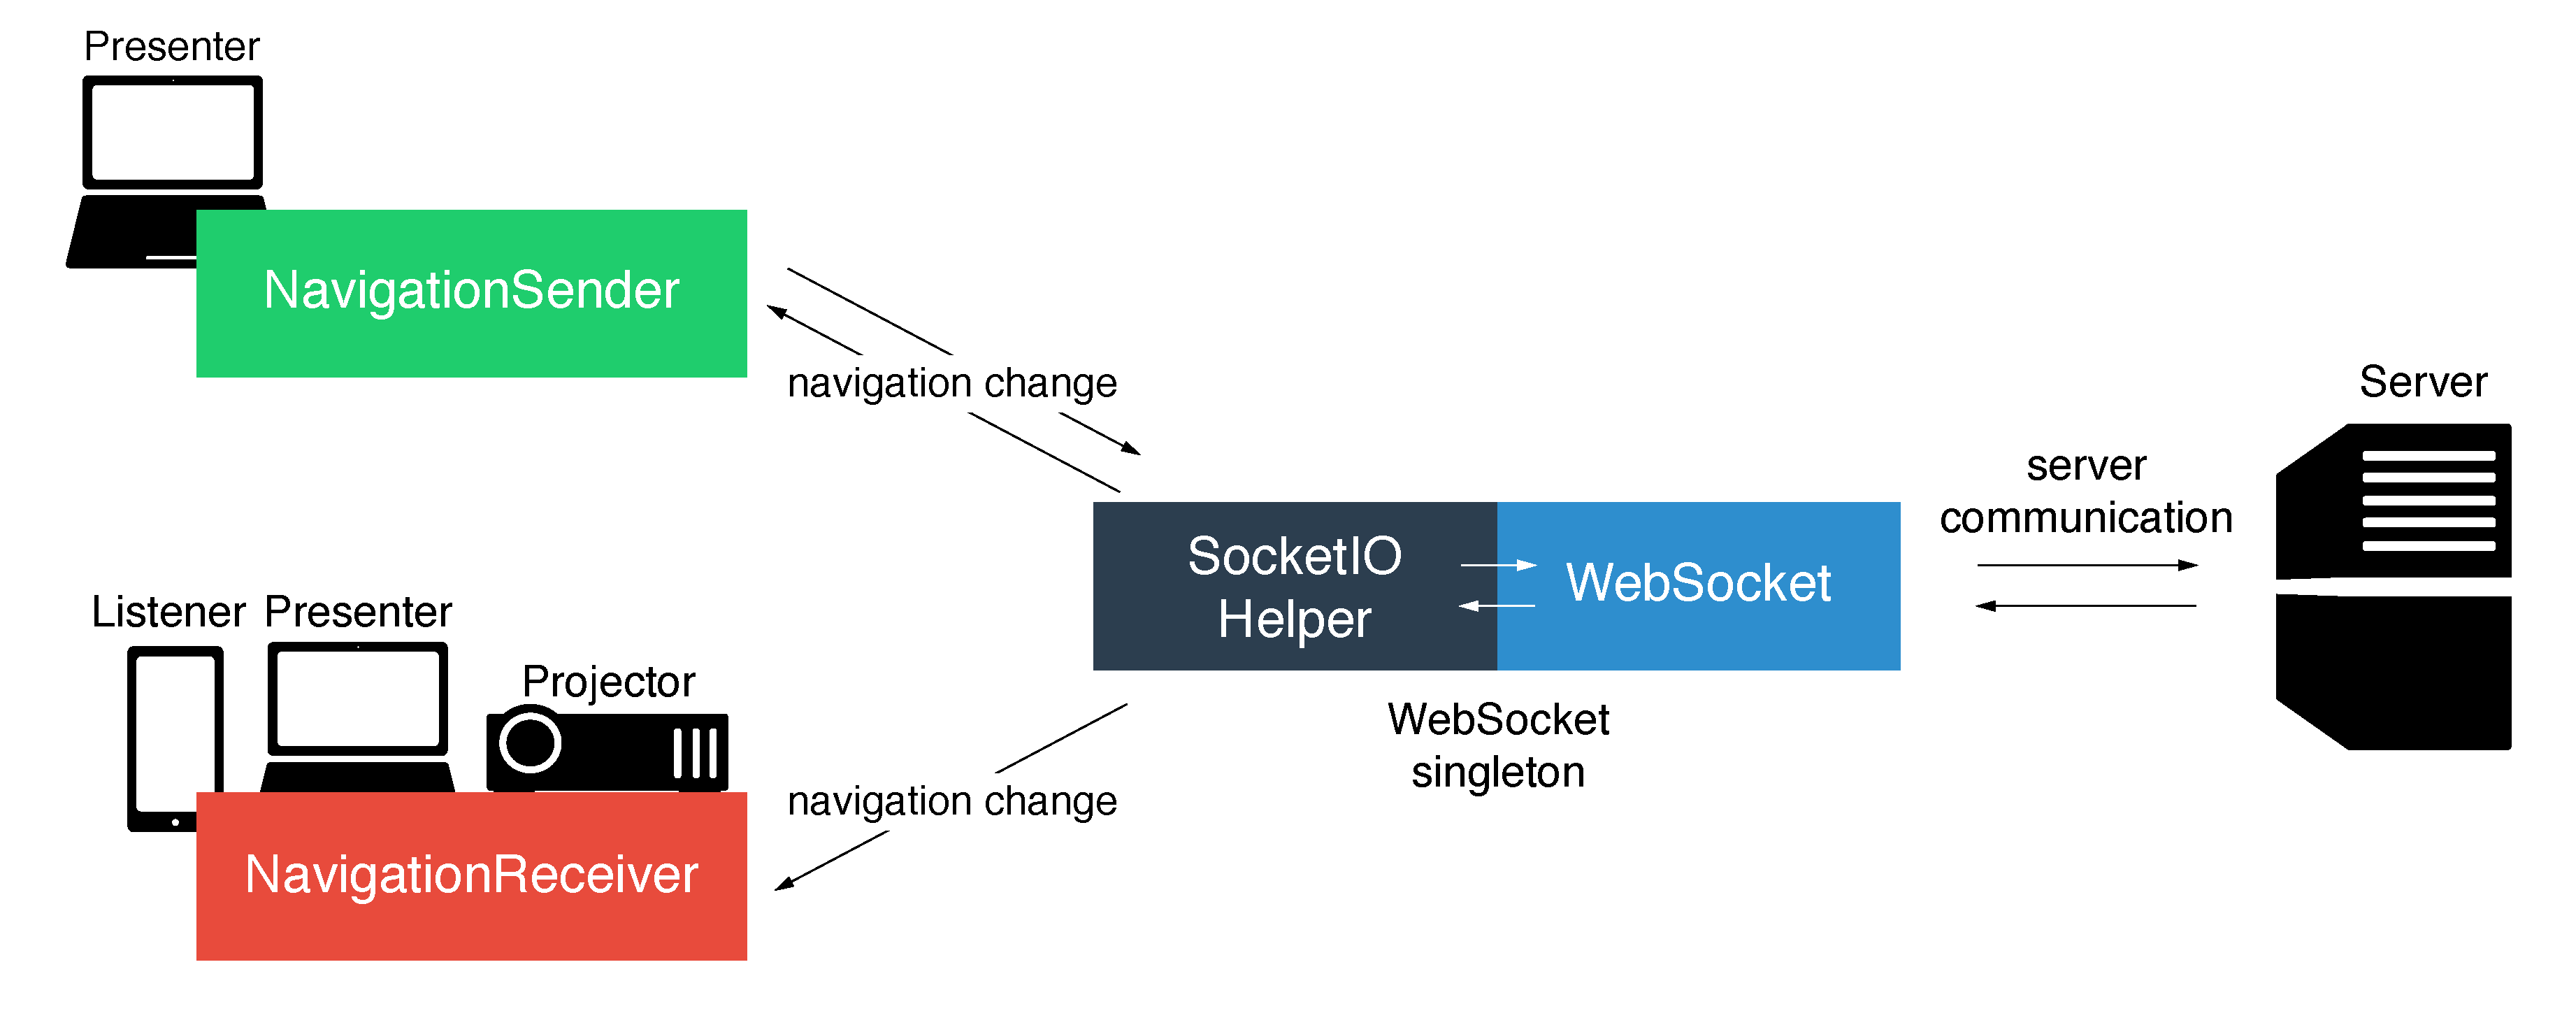
\includegraphics[width=1\textwidth]{network-sync}
\caption{Navigation synchronisation flow. \texttt{NavigationSender} emits a navigation change, which is sent to the server via WebSockets using the \texttt{SocketIO} helper and played back to the \texttt{NavigationReceiver} which is activated on all clients by default.}
\label{fig:implementation-network-sync}
\end{figure}

Besides providing a way of connecting to the server, this library also offers the components \texttt{NavigationSender} and \texttt{NavigationReceiver} for synchronising the navigation state of the presentation between speaker and audience. As the names already say, the sender broadcasts the state update, while the receiver is waiting for state updates and starts the navigation process. By default, the latter is active in all modes (default, speaker and projector), whereas the sender is only added to the speaker mode, effectively only broadcasting the speaker's navigation changes (see figure \ref{fig:implementation-network-sync}). To make sure the sender does not end up in an infinite loop of sending and receiving their own state changes, the last received state is stored and only navigation events going to a different slide are processed further.

This mechanism, though relatively simple, already enables the audience, and with that our listener Greg, to follow the presentation and the speaker Amy to use her phone or laptop as remote control for any number of connected projectors. Optionally, the \texttt{SynchronisableNavigationReceiver}, makes it possible to navigate entirely independently for listener and adds a button in the interface to switch back to the current presenter state.

\section{Interactive Extension}
\label{sec:implementation-interactive}

\begin{figure}
\centering
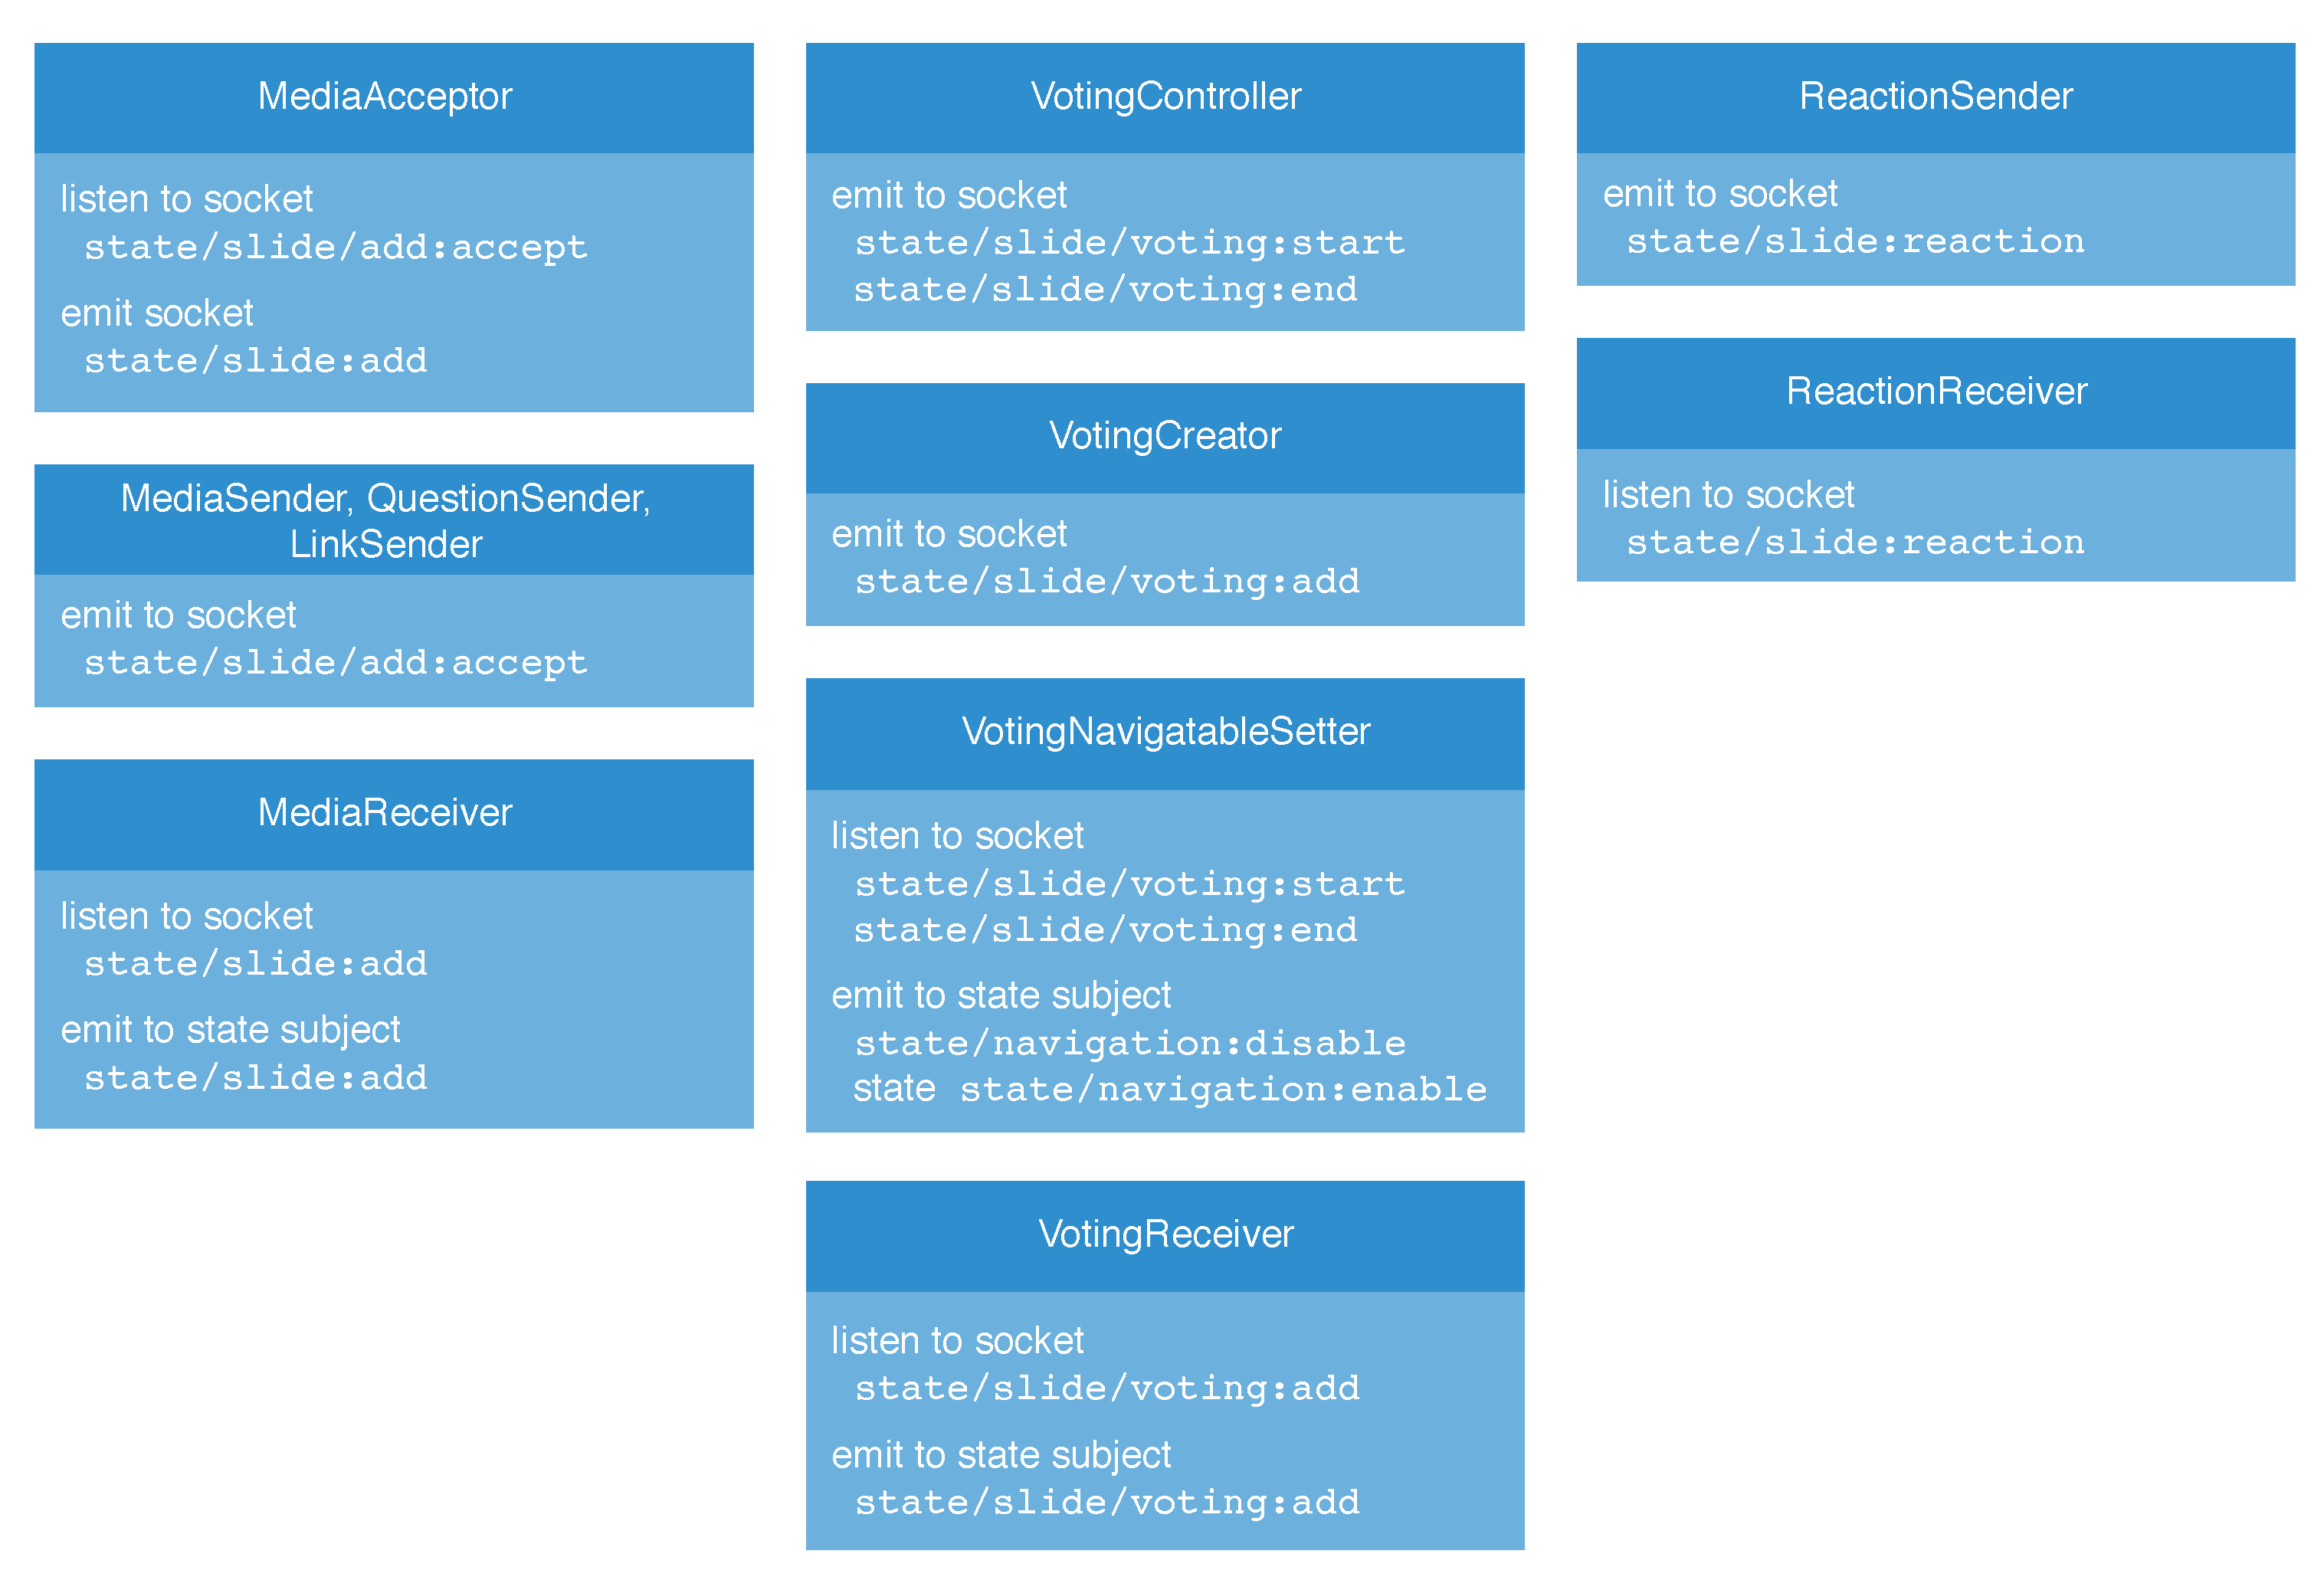
\includegraphics[width=\textwidth]{events-interactive}
\caption{Overview of state and socket events sent and consumed by controls in the interactive extension.}
\label{fig:implementation-events-interactive}
\end{figure}

The interactive library includes several parts which will be discussed here: a speaker presenter (section \ref{sec:implementation-interactive-speaker-presenter}) and different components connected to reactions (section \ref{sec:implementation-interactive-reactions}), sharing content (section \ref{sec:implementation-interactive-media}), and voting (section \ref{sec:implementation-interactive-voting}).

\subsection{Speaker Presenter}
\label{sec:implementation-interactive-speaker-presenter}

The speaker presenter, like the normal presenter, is responsible for rendering controls and slides. In speaker mode, where this presenter is used, notes as well as the upcoming slides (right and down) are also shown.
This means the presenter has to find these next slides, using the router's information about the navigatable directions, and render them in a designated area. As mentioned before, special attention was paid to mobile stylesheets to make the presenter view usable on mobile devices. This ensures that everything is big enough to be readable and all buttons are clickable (see figure \ref{fig:results-user-speaker-presenter}).

\subsection{Reactions}
\label{sec:implementation-interactive-reactions}
As with most other unveil library extensions described in here, the components for reactions also consist of a sender and a receiver: \texttt{ReactionSender} and \texttt{ReactionReceiver}. The principle is the same as with network synchronisation (see figure \ref{fig:implementation-network-sync}): When a listener chooses to send a reaction by clicking or tapping on an emoji, a \texttt{state/slide:reaction} is sent through the WebSocket. On the other side, the receiver is listening for the event and remembers which reactions have been sent on which slide, to display them. As a default, the sender is active in listener mode and the receiver is added to speaker and projector mode. On mobile, where the reactions are hidden behind a button and only slide in when tapping said button, a state-variable is responsible for storing the status of the reaction-picker. This works using CSS3 animations on the `max-height` attribute of the container.

\subsection{Content Sharing}
\label{sec:implementation-interactive-media}
Another responsibility of the interactive extension is the possibility for audience members to share content with the presentation. For this to work, five different controls were created: \texttt{MediaAcceptor}, \texttt{MediaReceiver} and the three senders \texttt{MediaSender}, \texttt{QuestionSender} and \texttt{LinkSender}. The senders are used in listener mode so members of the audience can share their content, the acceptor is enabled in speaker mode, to accept or reject incoming content and the receiver in the end handles the creation of a new slide if the content was accepted and is therefore necessary in all modes (see figure \ref{fig:implementation-interactive-media-pipeline}). As incoming content requests could disrupt the presentation flow and distract the speaker, an option to mute the requests was built into the application. If the \emph{do not disturb} mode is turned on, slides will silently be added as subslides, without causing the acceptor modal to open. This way the audience' additions can be re-visited after the end of the presentation. Generally, this feature can be used to either copy and paste a link to a picture, website or youtube video, for text input (i.e. questions) or to upload images directly from the listener's device. This works through the introduction of the presentation components \texttt{Media} and \texttt{IFrame}, which, depending on the shared content, render an image-tag, blockquote or IFrame. The differentiation of these is carried out using regular expressions. The native file upload works through the HTML5 File API, using \texttt{FileReader} \cite{file-api}. Once the file is uploaded, its contents are encoded as base64 data url and sent through the WebSocket.

As far as the implementation of the other controls is concerned, like the already discussed ones, they make use of the \texttt{SocketIO} helper to communicate with the server (see figure \ref{fig:implementation-events-interactive}). Additionally they use the \texttt{UnveilApp}'s state subject to start the process of adding a new slide. The sent \texttt{state/ slide:add} event includes details regarding where to add the new slide, its content, as well as how to add it (main or sub-slide). \texttt{UnveilApp} then inserts the new slide into the slide tree, re-computes the slide-map for the router and re-renders the entire presentation. The flow of the process is also outlined in figure \ref{fig:implementation-interactive-media-pipeline}.

The controls used for sharing content are also responsible for rendering the all necessary buttons and modals. The three senders render one \emph{share} button each, which toggles a \texttt{sharingMode} state variable and opens and closes the respective sharing modal. Something similar happens in the \texttt{MediaAcceptor}, which uses the \texttt{render()} method to display the \emph{mute} button and controls the modal for accepting new content, listening for incoming data. If a request arrives while another one has not yet been dealt with by the speaker, the request will be queued in the acceptor's interal state.

\begin{figure}
\centering
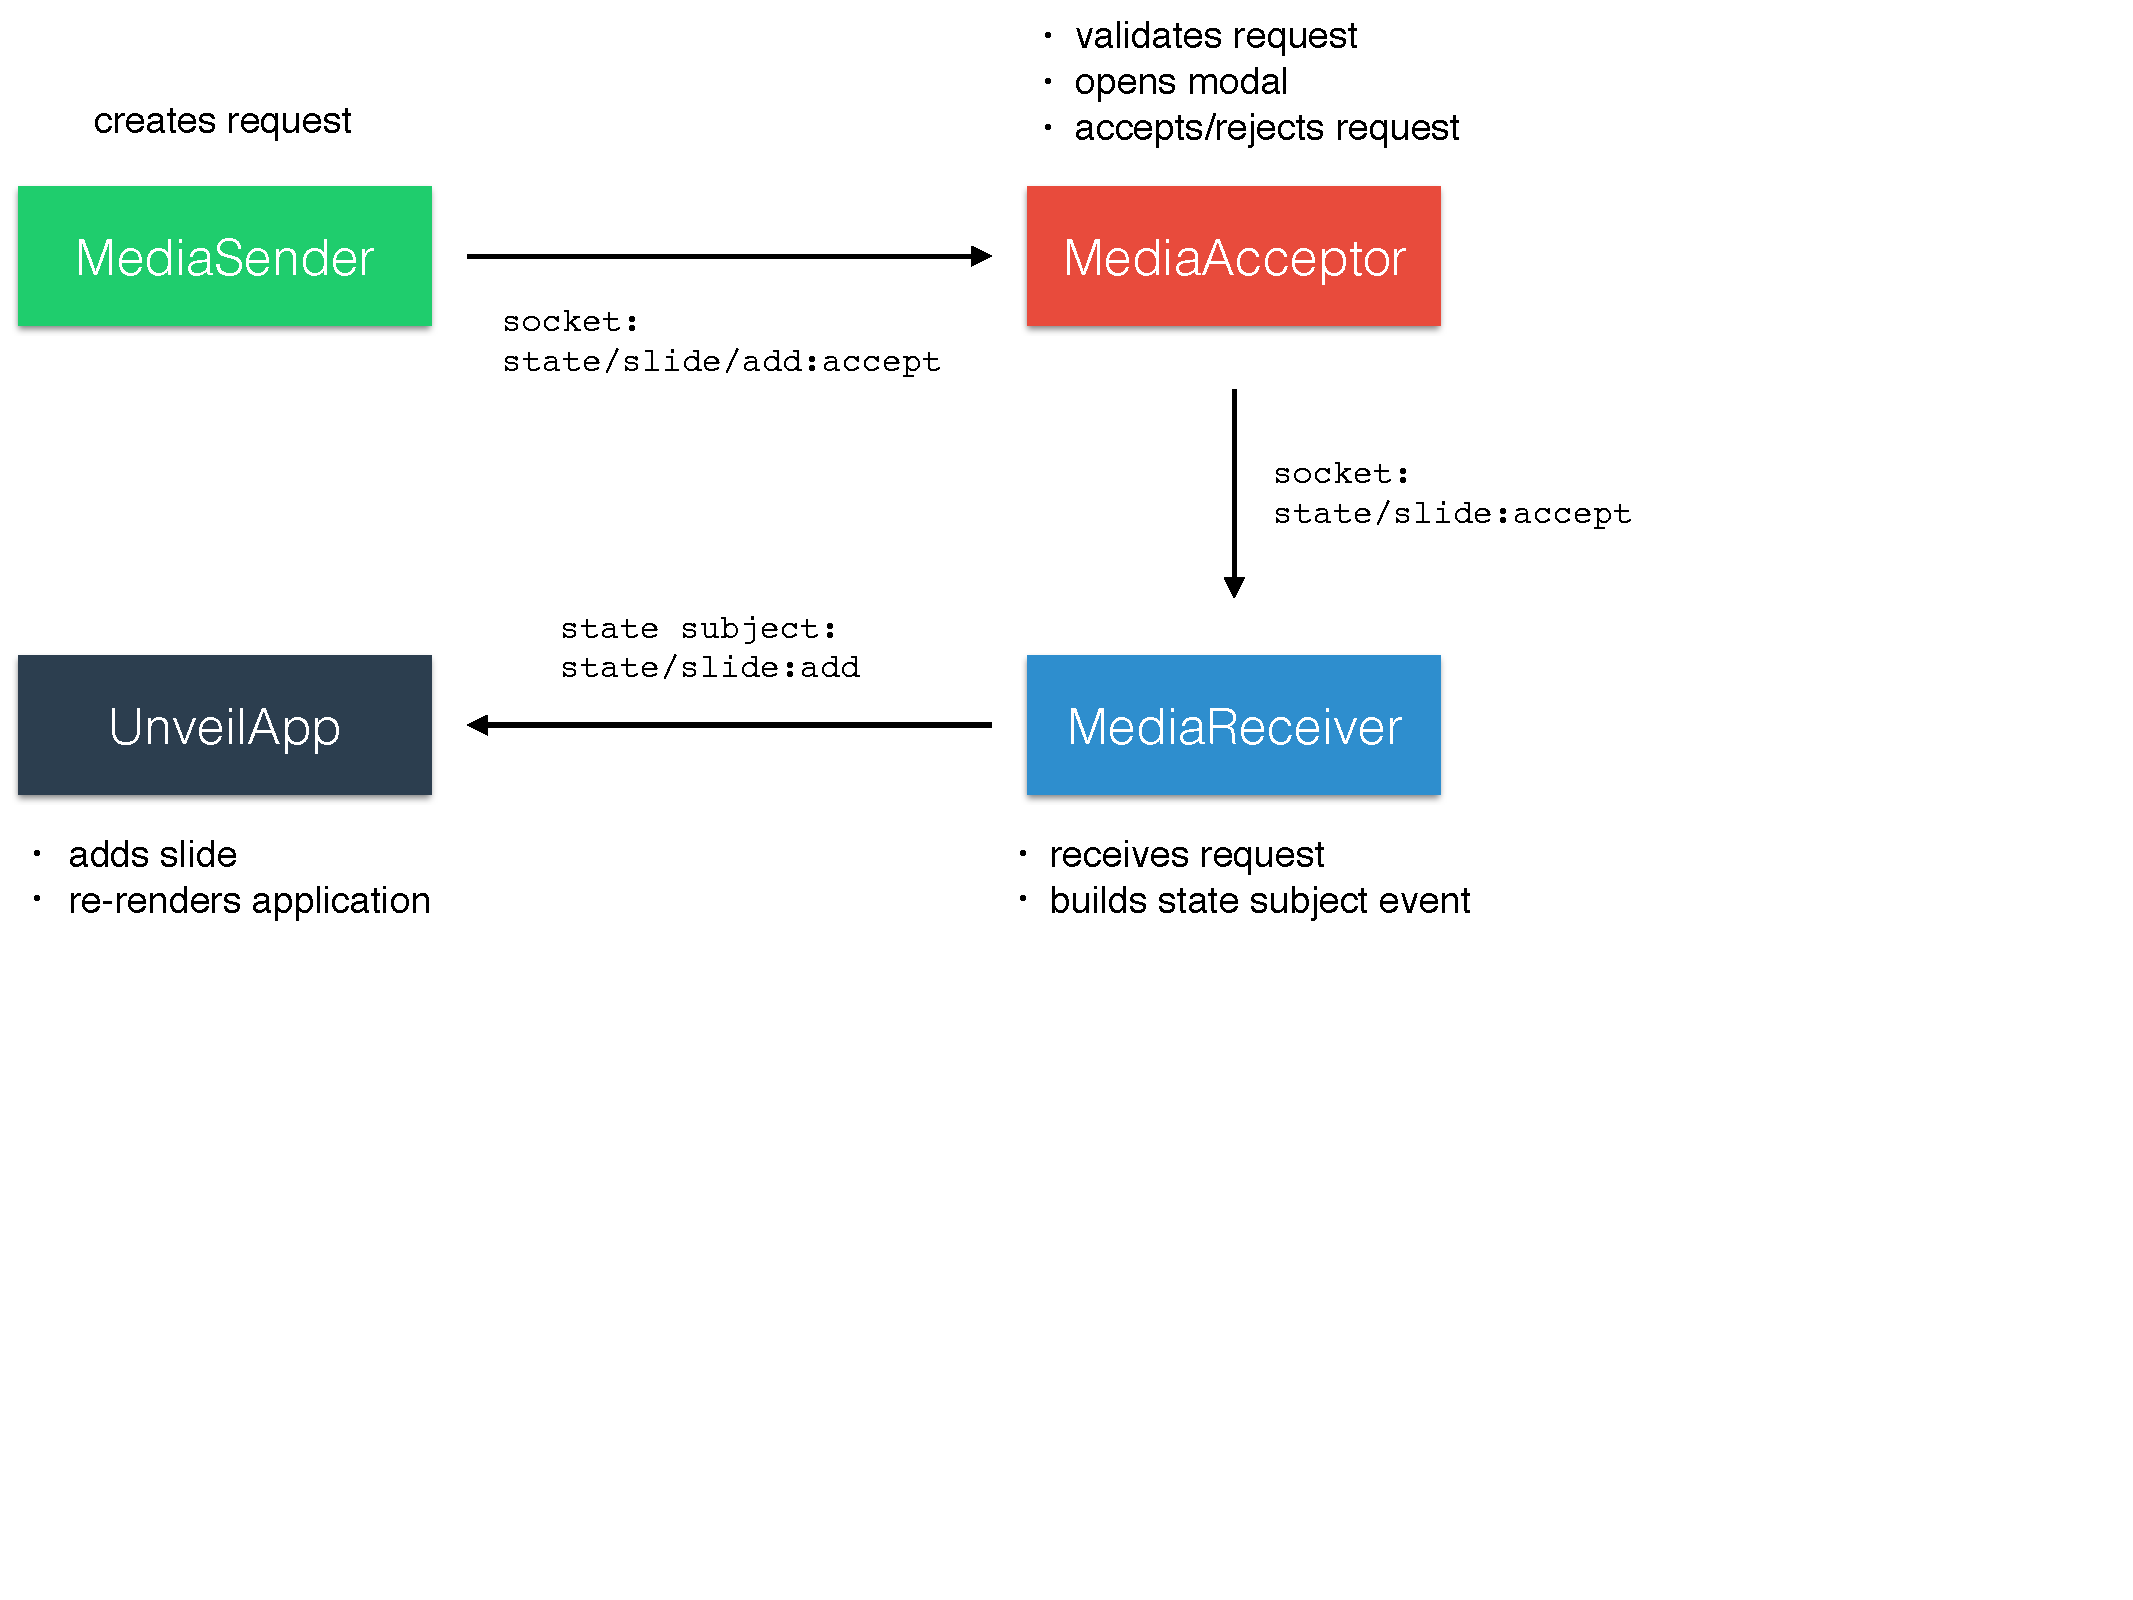
\includegraphics[width=1\textwidth]{media-pipeline}
\caption{Flow of adding content, monospaced text symbolises type and name of events. First the \texttt{MediaSender} of the listener mode sends a request, which the speaker mode's \texttt{MediaAcceptor} listens to. If the request is accepted by the speaker or requests are muted, another socket event is broadcast, which the \texttt{MediaReceiver} waits for. This component is enabled in all modes and emits the state subject event to add a new slide, which \texttt{UnveilApp} finally reacts to.}
\label{fig:implementation-interactive-media-pipeline}
\end{figure}

\subsection{Voting}
\label{sec:implementation-interactive-voting}

The last group of components connected to the interactive extension covered in this chapter allows speakers to create votings -- both during in the preparation of the presentation and on-the-fly -- and members of the audience to vote.

The main presentational component involved in the voting process is \texttt{Voting}, which keeps track of the current voting scores and has a \texttt{Question} and a number of \texttt{Answer} components as children. \texttt{Voting} also remembers if the current user has already voted and if so, displays the \texttt{Result}s instead of the form. In speaker and projector mode these results are shown at all times.

The audience can start submitting their votes as soon as the speaker navigates to the slide with the voting and until then the vote button is not rendered. Once the voting has started the possibility for all audience members to navigate to a different slide is disabled. The \texttt{VotingController} is active in speaker mode and checks the currently displayed slide for votings. If a new voting is active, the voting start event is emitted via the WebSocket. On the side of the audience, the \texttt{VotingNavigatableSetter} listens for this event as well as the voting end event and uses the state subject to enable and disable navigation in the presentation.

Once the voting has started, internally, the \texttt{Voting} component remembers which answer the user has clicked and once the submit button is pressed, fires a \texttt{state/slide/voting:answer} socket event. These in turn are used in the \texttt{Voting} components of the other clients to update the internal voting statistics. As the results of the voting should be available throughout the whole presentation and not be reset when leaving the slide, \texttt{Voting} also handles the communication with local storage, to persist the current results and voting status (voted or not). This happens in the update and mount lifecycle methods of the component using the name of the voting to identify the stored results. For votings created with the \texttt{VotingCreator}, this name is automatically created using the current timestamp. This component again renders a button in the speaker interface which toggles a modal. The creator internally stores a question and an array of answers, which can be filled in and added through the dialogue clicking the ``Create Voting'' button (see figure \ref{fig:results-user-polls-modal} in chapter \ref{cha:design}). This fires a socket event which the \texttt{VotingReceiver} is listening for to create a new slide from the sent details and start the adding process using unveil's state subject.

After discussing all important components of the developed application, it is time to have a look at how the library can be used and customised from the speaker's point of view.
